\documentclass[10pt,a4paper]{article}
\usepackage[margin=21mm,headheight=15pt]{geometry}
\usepackage[T1]{fontenc}
\usepackage{lmodern,amsmath,amssymb,tikz,graphicx,hyperref,fancyhdr,enumitem}
\usetikzlibrary{arrows.meta,positioning,calc,decorations.pathmorphing}
\definecolor{ink}{RGB}{20,53,78}
\hypersetup{colorlinks=true,urlcolor=ink,linkcolor=ink}
\setlength{\parindent}{0pt}\setlength{\parskip}{5pt}
\emergencystretch=3em
\pagestyle{fancy}\fancyhf{}\fancyfoot[C]{\thepage}
\renewcommand{\headrulewidth}{.3pt}
\newcommand{\task}[2]{\par\medskip{\color{ink}\Large\bfseries #1. #2}\par\smallskip}
\newcommand{\answer}{\par\smallskip\textbf{Worked reasoning.} }
\setlist[enumerate]{label=\textbf{(\alph*)},leftmargin=7mm,itemsep=7pt}
\begin{document}
\fancyhead[L]{\small Control of Dynamical Systems}
\fancyhead[R]{\small Illustrated models}
{\Huge\color{ink}\bfseries Physical systems and control models}\par
Original vector illustrations for the hypothetical learning collection. Equipment views identify the modeled phenomenon; signal diagrams identify its mathematical structure. A picture does not establish experimental validation.
\section*{01. Thermal enclosure and a slow sensor}
\begin{center}\resizebox{\ifdim\width>.98\linewidth.98\linewidth\else\width\fi}{!}{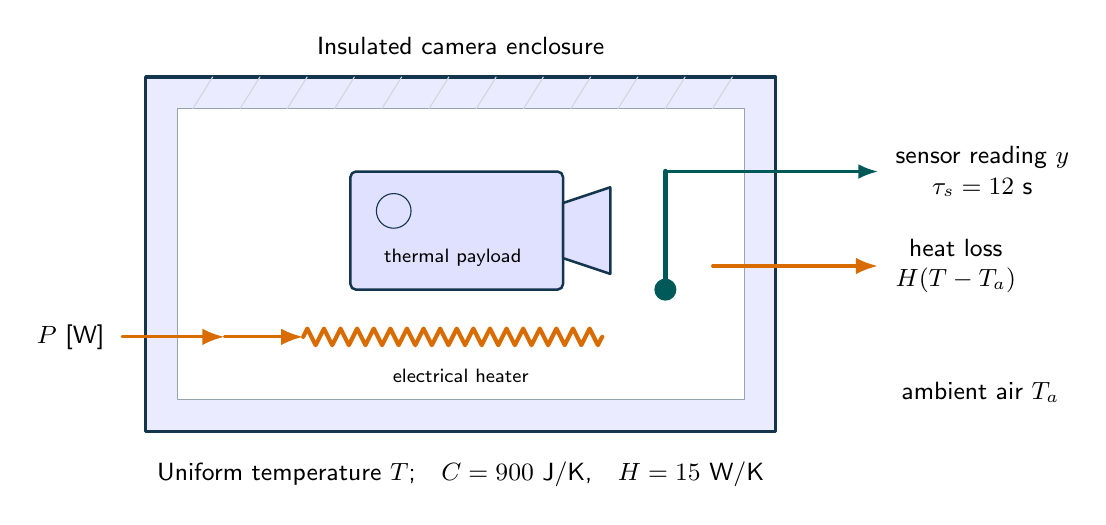
\begin{tikzpicture}[
font=\sffamily\small,>=Latex,line cap=round,line join=round,
wall/.style={draw=ink,line width=1.2pt,fill=blue!5},
water/.style={fill=cyan!25,draw=none},
metal/.style={draw=ink,fill=blue!12,line width=.9pt},
flow/.style={->,draw=blue!65!black,line width=1.2pt},
heat/.style={->,draw=orange!85!black,line width=1.1pt},
measure/.style={->,draw=teal!70!black,line width=.9pt},
dim/.style={<->,draw=ink!65,line width=.6pt},
spring/.style={draw=ink,decorate,decoration={coil,aspect=.5,segment length=4pt,amplitude=3pt}},
wire/.style={draw=ink,line width=1pt},
lab/.style={align=center,font=\sffamily\small},
smalllab/.style={align=center,font=\sffamily\scriptsize}]

\fill[blue!8] (1,0) rectangle (9,4.5);
\fill[white] (1.4,.4) rectangle (8.6,4.1);
\draw[ink,line width=1.2pt] (1,0) rectangle (9,4.5);
\draw[ink!45] (1.4,.4) rectangle (8.6,4.1);
\foreach \x in {1.6,2.2,...,8.2}{\draw[ink!20](\x,4.1)--++(.25,.4);}
\node[lab]at(5,4.9){Insulated camera enclosure};
\draw[metal,rounded corners=2pt](3.6,1.8)rectangle(6.3,3.3);
\draw[metal](6.3,2.2)--(6.9,2)--(6.9,3.1)--(6.3,2.9)--cycle;
\draw[ink](4.15,2.8)circle(.22);
\node[smalllab]at(4.9,2.2){thermal payload};
\draw[heat](2,1.2)--(3,1.2);
\draw[orange!85!black,line width=1.5pt,decorate,decoration={zigzag,segment length=6pt,amplitude=3pt}](3,1.2)--(6.8,1.2);
\node[lab,anchor=east]at(.6,1.2){$P$ [W]};
\draw[heat](.7,1.2)--(2,1.2);
\node[smalllab]at(5,.7){electrical heater};
\draw[teal!70!black,line width=2pt](7.6,1.8)--(7.6,3.3);
\fill[teal!70!black](7.6,1.8)circle(.14);
\draw[measure](7.6,3.3)--(10.3,3.3);
\node[lab,anchor=west]at(10.4,3.3){sensor reading $y$\\$\tau_s=12$ s};
\draw[heat](8.2,2.1)--(10.3,2.1);
\node[lab,anchor=west]at(10.4,2.1){heat loss\\$H(T-T_a)$};
\node[lab]at(11.6,.5){ambient air $T_a$};
\node[lab]at(5,-.55){Uniform temperature $T$;\quad $C=900$ J/K,\quad $H=15$ W/K};
\end{tikzpicture}
}\par{\small Cutaway of a lumped thermal enclosure. Orange arrows carry heat; the probe measures a lagged temperature. The drawing fixes the energy boundary, not a real device geometry.}\end{center}
\medskip\textbf{From equipment to equations}\par
\begin{center}\resizebox{\ifdim\width>.98\linewidth.98\linewidth\else\width\fi}{!}{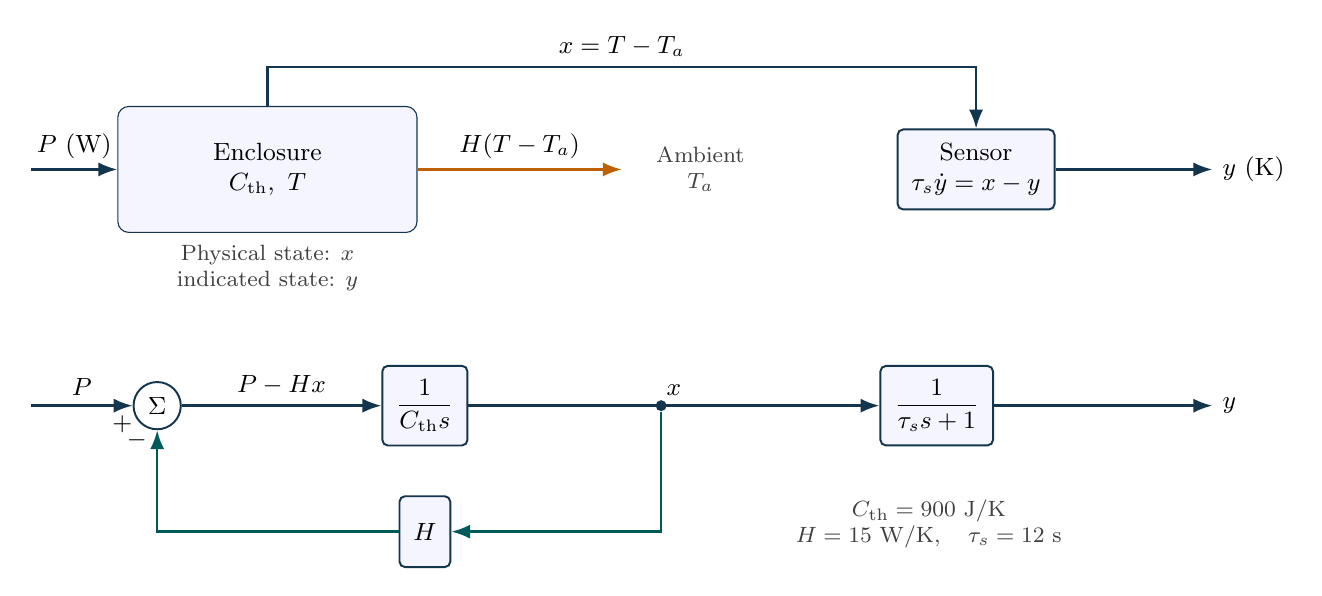
\begin{tikzpicture}[x=1cm,y=1cm,>=Latex,font=\small,
block/.style={draw=ink,fill=blue!4,rounded corners=2pt,minimum height=9mm,align=center,line width=.7pt,inner sep=5pt},
sum/.style={circle,draw=ink,fill=white,minimum size=6mm,inner sep=0pt,line width=.7pt},
sig/.style={->,draw=ink,line width=.85pt},
fb/.style={->,draw=teal!70!black,line width=.85pt},
dist/.style={->,draw=orange!75!black,line width=.85pt},
tap/.style={circle,fill=ink,inner sep=1.4pt},
note/.style={font=\footnotesize,align=center,text=black!75}]

\node[draw=ink,fill=blue!4,rounded corners,minimum width=38mm,minimum height=16mm,align=center](en)at(3,2.5){Enclosure\\$C_{\mathrm{th}},\ T$};
\draw[sig](0,2.5)--node[above]{$P$ (W)}(en.west);
\draw[dist](en.east)--node[above]{$H(T-T_a)$}(7.5,2.5);
\node[note]at(8.5,2.5){Ambient\\$T_a$};
\node[block](sensor)at(12,2.5){Sensor\\$\tau_s\dot y=x-y$};
\draw[sig](en.north)--(3,3.8)--node[above]{$x=T-T_a$}(12,3.8)--(sensor.north);
\draw[sig](sensor.east)--(15,2.5)node[right]{$y$ (K)};
\node[note]at(3,1.25){Physical state: $x$\\indicated state: $y$};
\node[sum](s)at(1.6,-.5){$\Sigma$};
\node[block](int)at(5,-.5){$\dfrac{1}{C_{\mathrm{th}}s}$};
\node[tap](xt)at(8,-.5){};
\node[block](gs)at(11.5,-.5){$\dfrac{1}{\tau_s s+1}$};
\draw[sig](0,-.5)--node[above]{$P$}node[pos=.9,below]{$+$}(s);
\draw[sig](s)--node[above]{$P-Hx$}(int);
\draw[sig](int)--node[above]{$x$}(gs);
\draw[sig](gs)--(15,-.5)node[right]{$y$};
\node[block](h)at(5,-2.1){$H$};
\draw[fb](xt)--(8,-2.1)--(h);
\draw[fb](h)--(1.6,-2.1)--node[pos=.9,left]{$-$}(s);
\node[note]at(11.4,-2){$C_{\mathrm{th}}=900\ \mathrm{J/K}$\\$H=15\ \mathrm{W/K},\quad\tau_s=12\ \mathrm{s}$};

\end{tikzpicture}
}\par{\small Thermal storage, heat leakage and sensor dynamics are separate elements. The lower loop implements the energy balance, not an added temperature controller.}\end{center}

\newpage
\section*{02. Ventilation as a bilinear dynamical system}
\begin{center}\resizebox{\ifdim\width>.98\linewidth.98\linewidth\else\width\fi}{!}{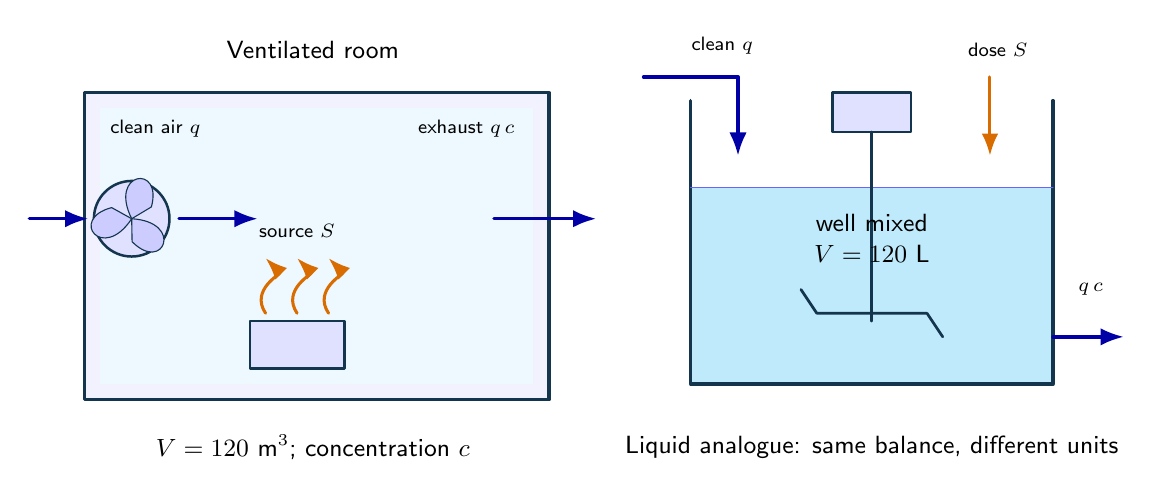
\begin{tikzpicture}[
font=\sffamily\small,>=Latex,line cap=round,line join=round,
wall/.style={draw=ink,line width=1.2pt,fill=blue!5},
water/.style={fill=cyan!25,draw=none},
metal/.style={draw=ink,fill=blue!12,line width=.9pt},
flow/.style={->,draw=blue!65!black,line width=1.2pt},
heat/.style={->,draw=orange!85!black,line width=1.1pt},
measure/.style={->,draw=teal!70!black,line width=.9pt},
dim/.style={<->,draw=ink!65,line width=.6pt},
spring/.style={draw=ink,decorate,decoration={coil,aspect=.5,segment length=4pt,amplitude=3pt}},
wire/.style={draw=ink,line width=1pt},
lab/.style={align=center,font=\sffamily\small},
smalllab/.style={align=center,font=\sffamily\scriptsize}]

\draw[wall](.3,.2)--(.3,4.1)--(6.2,4.1)--(6.2,.2)--cycle;
\fill[cyan!7](.5,.4)rectangle(6,3.9);
\draw[metal](.9,2.5)circle(.48);
\foreach \a in {0,120,240}{\draw[ink,fill=blue!20,rotate around={\a:(.9,2.5)}](.9,2.5)..controls(.6,3.1)and(1.3,3.2)..(1.15,2.65)--cycle;}
\draw[flow](-.4,2.5)--(.35,2.5);
\draw[flow](1.5,2.5)--(2.5,2.5);
\draw[flow](5.5,2.5)--(6.8,2.5);
\node[smalllab]at(1.2,3.65){clean air $q$};
\node[smalllab]at(5.15,3.65){exhaust $q\,c$};
\draw[metal](2.4,.6)rectangle(3.6,1.2);
\foreach \x in {2.6,3,3.4}{\draw[heat](\x,1.3)..controls(\x-.2,1.6)and(\x+.2,1.8)..(\x,2);}
\node[smalllab]at(3,2.35){source $S$};
\node[lab]at(3.2,4.65){Ventilated room};
\node[lab]at(3.2,-.4){$V=120$ m$^3$; concentration $c$};
\fill[water](8,.4)rectangle(12.6,2.9);
\draw[wall,fill=none](8,4)--(8,.4)--(12.6,.4)--(12.6,4);
\draw[blue!60](8,2.9)--(12.6,2.9);
\draw[flow](7.4,4.3)--(8.6,4.3)--(8.6,3.3);
\draw[flow](12.6,1)--(13.5,1);
\draw[metal](9.8,3.6)rectangle(10.8,4.1);
\draw[wire](10.3,3.6)--(10.3,1.2);
\draw[wire](9.6,1.3)--(11,1.3)(9.6,1.3)--(9.4,1.6)(11,1.3)--(11.2,1);
\draw[heat](11.8,4.3)--(11.8,3.3);
\node[smalllab]at(11.9,4.65){dose $S$};
\node[smalllab]at(8.4,4.7){clean $q$};
\node[smalllab,anchor=west]at(12.8,1.6){$q\,c$};
\node[lab]at(10.3,2.25){well mixed\\$V=120$ L};
\node[lab]at(10.3,-.4){Liquid analogue: same balance, different units};
\end{tikzpicture}
}\par{\small A ventilated room and a well-mixed liquid analogue share an inventory balance. The room uses m$^3$ and the liquid case uses L; do not mix their concentration or flow units. Equal inlet and outlet volume flows keep each inventory constant.}\end{center}
\medskip\textbf{From equipment to equations}\par
\begin{center}\resizebox{\ifdim\width>.98\linewidth.98\linewidth\else\width\fi}{!}{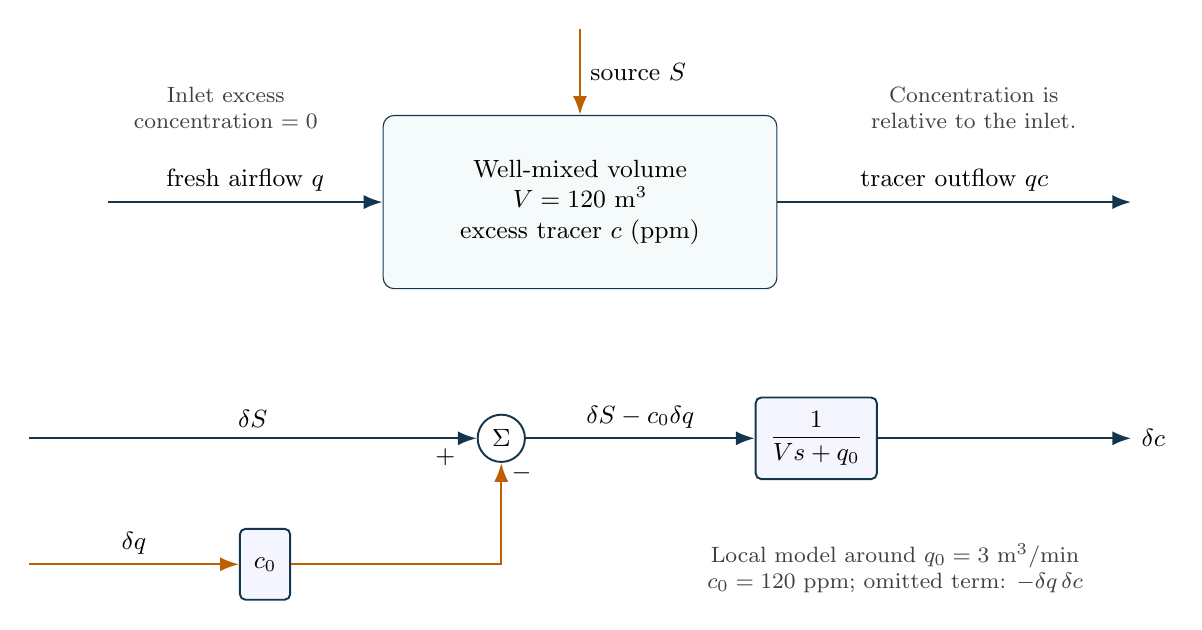
\begin{tikzpicture}[x=1cm,y=1cm,>=Latex,font=\small,
block/.style={draw=ink,fill=blue!4,rounded corners=2pt,minimum height=9mm,align=center,line width=.7pt,inner sep=5pt},
sum/.style={circle,draw=ink,fill=white,minimum size=6mm,inner sep=0pt,line width=.7pt},
sig/.style={->,draw=ink,line width=.85pt},
fb/.style={->,draw=teal!70!black,line width=.85pt},
dist/.style={->,draw=orange!75!black,line width=.85pt},
tap/.style={circle,fill=ink,inner sep=1.4pt},
note/.style={font=\footnotesize,align=center,text=black!75}]

\node[draw=ink,fill=teal!4,rounded corners,minimum width=50mm,minimum height=22mm,align=center](v)at(7,2.3){Well-mixed volume\\$V=120\ \mathrm{m^3}$\\excess tracer $c$ (ppm)};
\draw[sig](1,2.3)--node[above]{fresh airflow $q$}(v.west);
\draw[sig](v.east)--node[above]{tracer outflow $qc$}(14,2.3);
\draw[dist](7,4.5)--node[right]{source $S$}(v.north);
\node[note]at(2.5,3.5){Inlet excess\\concentration $=0$};
\node[note]at(12,3.5){Concentration is\\relative to the inlet.};
\node[sum](s)at(6,-.7){$\Sigma$};
\node[block](p)at(10,-.7){$\dfrac{1}{Vs+q_0}$};
\node[block](gain)at(3,-2.3){$c_0$};
\draw[sig](0,-.7)--node[above]{$\delta S$}node[pos=.93,below]{$+$}(s);
\draw[dist](0,-2.3)--node[above]{$\delta q$}(gain);
\draw[dist](gain)--(6,-2.3)--node[pos=.9,right]{$-$}(s);
\draw[sig](s)--node[above]{$\delta S-c_0\delta q$}(p);
\draw[sig](p)--(14,-.7)node[right]{$\delta c$};
\node[note]at(11,-2.35){Local model around $q_0=3\ \mathrm{m^3/min}$\\$c_0=120\ \mathrm{ppm}$; omitted term: $-\delta q\,\delta c$};

\end{tikzpicture}
}\par{\small The physical balance and its local two-input signal model. Airflow enters with a negative sign because increased ventilation removes excess tracer.}\end{center}

\newpage
\section*{03. A precision platform under floor motion}
\begin{center}\resizebox{\ifdim\width>.98\linewidth.98\linewidth\else\width\fi}{!}{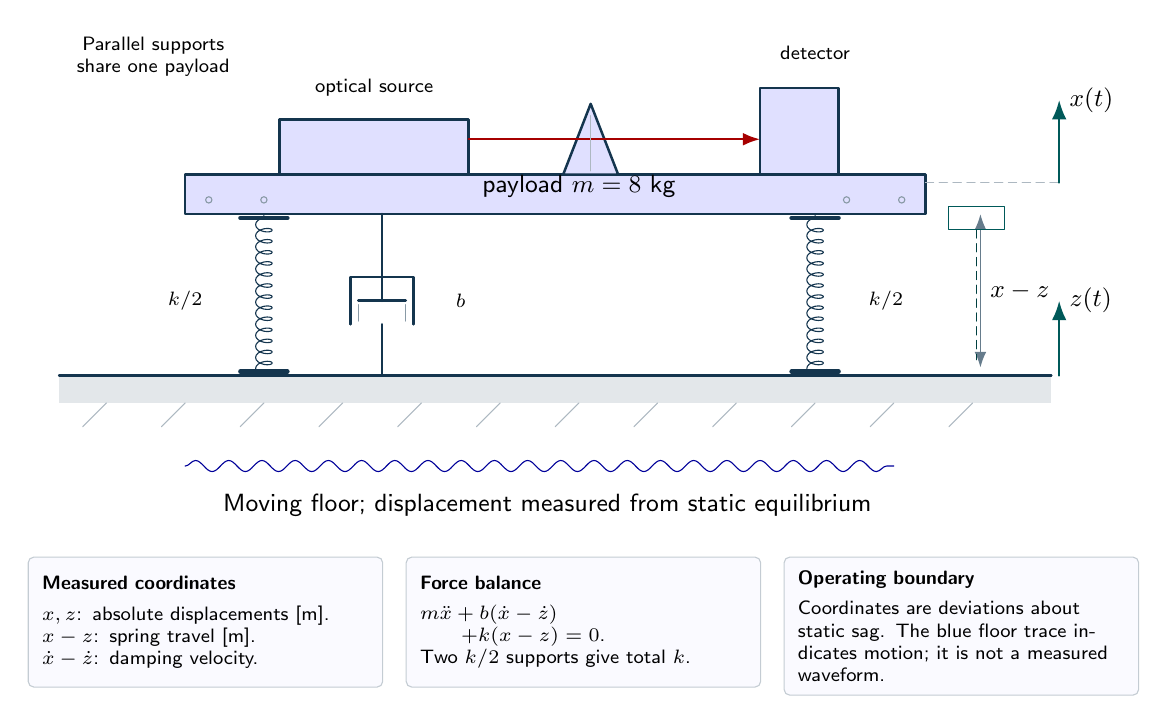
\begin{tikzpicture}[
font=\sffamily\small,>=Latex,line cap=round,line join=round,
wall/.style={draw=ink,line width=1.2pt,fill=blue!5},
water/.style={fill=cyan!25,draw=none},
metal/.style={draw=ink,fill=blue!12,line width=.9pt},
flow/.style={->,draw=blue!65!black,line width=1.2pt},
heat/.style={->,draw=orange!85!black,line width=1.1pt},
measure/.style={->,draw=teal!70!black,line width=.9pt},
dim/.style={<->,draw=ink!65,line width=.6pt},
spring/.style={draw=ink,decorate,decoration={coil,aspect=.5,segment length=4pt,amplitude=3pt}},
wire/.style={draw=ink,line width=1pt},
lab/.style={align=center,font=\sffamily\small},
smalllab/.style={align=center,font=\sffamily\scriptsize}]

\fill[ink!12](.4,.2)rectangle(13,.55);
\draw[ink,line width=1pt](.4,.55)--(13,.55);
\foreach \x in {1,2,...,12}{\draw[ink!35](\x,.2)--++(-.3,-.3);}
\draw[metal](2,2.6)rectangle(11.4,3.1);
\draw[spring](3,.55)--(3,2.6);
\draw[spring](10,.55)--(10,2.6);
\draw[wire](4.5,.55)--(4.5,1.2)(4.1,1.2)--(4.1,1.8)--(4.9,1.8)--(4.9,1.2);
\draw[wire](4.5,2.6)--(4.5,1.5)(4.2,1.5)--(4.8,1.5);
\draw[metal](3.2,3.1)rectangle(5.6,3.8);
\draw[metal](6.8,3.1)--(7.15,4)--(7.5,3.1)--cycle;
\draw[metal](9.3,3.1)rectangle(10.3,4.2);
\draw[red!65!black,->,line width=.7pt](5.6,3.55)--(9.3,3.55);
\node[smalllab]at(4.4,4.2){optical source};
\node[smalllab]at(10,4.65){detector};
\node[lab]at(7,2.95){payload $m=8$ kg};
\node[smalllab]at(2,1.5){$k/2$};\node[smalllab]at(10.9,1.5){$k/2$};
\node[smalllab]at(5.5,1.5){$b$};
\draw[dim](12.1,.65)--node[right]{$x-z$}(12.1,2.6);
\draw[ink!35,densely dashed](11.4,3)--(13.1,3);
\draw[measure](13.1,3)--(13.1,4.05)node[right]{$x(t)$};
\draw[measure](13.1,.55)--(13.1,1.5)node[right]{$z(t)$};
\draw[blue!60!black,decorate,decoration={snake,amplitude=2pt,segment length=12pt}](2,-.6)--(11,-.6);
\node[lab]at(6.6,-1.1){Moving floor; displacement measured from static equilibrium};
% REFINED EQUIPMENT DETAILS

% Fasteners, spring seats and a clearly resolved dashpot piston.
\foreach \x in {2.3,3,10.4,11.1}{\draw[ink!50](\x,2.78)circle(.04);}
\foreach \x in {3,10}{\draw[ink,line width=1.5pt](\x-.3,.6)--(\x+.3,.6)(\x-.3,2.55)--(\x+.3,2.55);}
\draw[ink!50](4.2,1.24)--(4.2,1.45)(4.8,1.24)--(4.8,1.45);
\draw[ink!35](7.15,3.15)--(7.15,3.85);
\draw[teal!70!black](11.7,2.4)rectangle(12.4,2.7);
\draw[teal!50!black,densely dashed](12.05,2.4)--(12.05,.75);
\node[smalllab,anchor=west]at(.5,4.6){Parallel supports\\share one payload};

\node[draw=ink!25,fill=blue!2,rounded corners=2pt,anchor=north west,text width=4.15cm,minimum height=1.65cm,inner sep=5pt,align=left,font=\sffamily\scriptsize]at(0.0,-1.75){\textbf{Measured coordinates}\\[3pt]$x,z$: absolute displacements [m].\\$x-z$: spring travel [m].\\$\dot x-\dot z$: damping velocity.};
\node[draw=ink!25,fill=blue!2,rounded corners=2pt,anchor=north west,text width=4.15cm,minimum height=1.65cm,inner sep=5pt,align=left,font=\sffamily\scriptsize]at(4.8,-1.75){\textbf{Force balance}\\[3pt]$m\ddot x+b(\dot x-\dot z)$\\$\qquad+k(x-z)=0$.\\Two $k/2$ supports give total $k$.};
\node[draw=ink!25,fill=blue!2,rounded corners=2pt,anchor=north west,text width=4.15cm,minimum height=1.65cm,inner sep=5pt,align=left,font=\sffamily\scriptsize]at(9.6,-1.75){\textbf{Operating boundary}\\[3pt]Coordinates are deviations about static sag. The blue floor trace indicates motion; it is not a measured waveform.};
\end{tikzpicture}
}\par{\small An optical payload rests on parallel spring and damping elements. The two springs each have stiffness $k/2$, giving total $k$. Both the floor and payload move; spring extension and damping velocity are relative quantities. Weight is balanced at the static equilibrium about which the model is written.}\end{center}
\medskip\textbf{From equipment to equations}\par
\begin{center}\resizebox{\ifdim\width>.98\linewidth.98\linewidth\else\width\fi}{!}{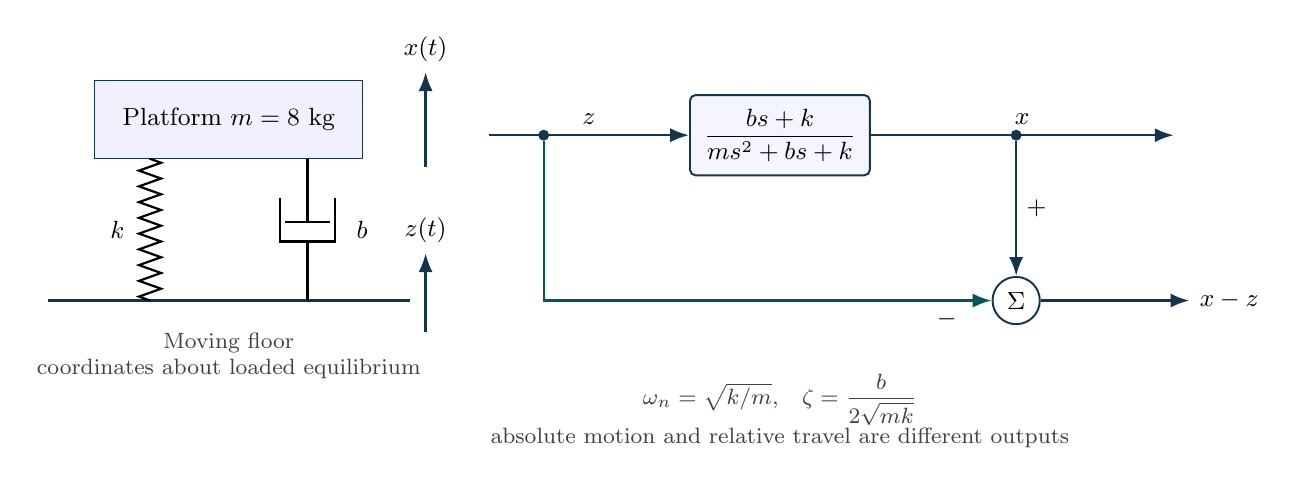
\begin{tikzpicture}[x=1cm,y=1cm,>=Latex,font=\small,
block/.style={draw=ink,fill=blue!4,rounded corners=2pt,minimum height=9mm,align=center,line width=.7pt,inner sep=5pt},
sum/.style={circle,draw=ink,fill=white,minimum size=6mm,inner sep=0pt,line width=.7pt},
sig/.style={->,draw=ink,line width=.85pt},
fb/.style={->,draw=teal!70!black,line width=.85pt},
dist/.style={->,draw=orange!75!black,line width=.85pt},
tap/.style={circle,fill=ink,inner sep=1.4pt},
note/.style={font=\footnotesize,align=center,text=black!75}]

\node[draw=ink,fill=blue!6,minimum width=34mm,minimum height=10mm](m)at(2,2.2){Platform $m=8$ kg};
\draw[line width=1.2pt,draw=ink](-.3,-.1)--(4.3,-.1);
\draw[decorate,decoration={zigzag,segment length=2mm,amplitude=1.4mm},line width=.8pt](1,-.1)--(1,1.7);
\node[left]at(.8,.8){$k$};
\draw[line width=.8pt](3,-.1)--(3,.65);
\draw[line width=.8pt](2.65,1.2)--(2.65,.65)--(3.35,.65)--(3.35,1.2);
\draw[line width=.8pt](2.72,.9)--(3.28,.9);
\draw[line width=.8pt](3,.9)--(3,1.7);
\node[right]at(3.5,.8){$b$};
\draw[sig](4.5,1.6)--(4.5,2.8)node[above]{$x(t)$};
\draw[sig](4.5,-.5)--(4.5,.5)node[above]{$z(t)$};
\node[note]at(2,-.8){Moving floor\\coordinates about loaded equilibrium};
\node[block](g)at(9,2){$\dfrac{bs+k}{ms^2+bs+k}$};
\node[tap](zt)at(6,2){};
\node[tap](xt)at(12,2){};
\draw[sig](5.3,2)--node[above]{$z$}(g);
\draw[sig](g)--node[above]{$x$}(14,2);
\node[sum](rel)at(12,-.1){$\Sigma$};
\draw[sig](xt)--node[right]{$+$}(rel);
\draw[fb](zt)--(6,-.1)--node[pos=.9,below]{$-$}(rel);
\draw[sig](rel)--(14.2,-.1)node[right]{$x-z$};
\node[note]at(9,-1.5){$\omega_n=\sqrt{k/m}$,\quad $\zeta=\dfrac{b}{2\sqrt{mk}}$\\absolute motion and relative travel are different outputs};

\end{tikzpicture}
}\par{\small Base excitation drives absolute motion; subtracting the floor coordinate gives relative travel. The spring and damper act in parallel.}\end{center}

\newpage
\section*{04. A passive notch filter and component tolerance}
\begin{center}\resizebox{\ifdim\width>.98\linewidth.98\linewidth\else\width\fi}{!}{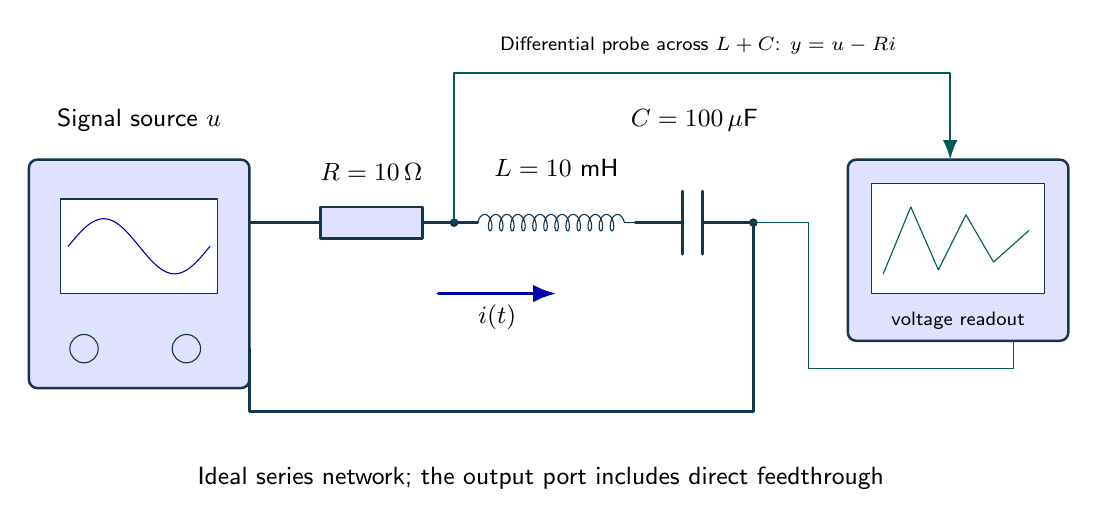
\begin{tikzpicture}[
font=\sffamily\small,>=Latex,line cap=round,line join=round,
wall/.style={draw=ink,line width=1.2pt,fill=blue!5},
water/.style={fill=cyan!25,draw=none},
metal/.style={draw=ink,fill=blue!12,line width=.9pt},
flow/.style={->,draw=blue!65!black,line width=1.2pt},
heat/.style={->,draw=orange!85!black,line width=1.1pt},
measure/.style={->,draw=teal!70!black,line width=.9pt},
dim/.style={<->,draw=ink!65,line width=.6pt},
spring/.style={draw=ink,decorate,decoration={coil,aspect=.5,segment length=4pt,amplitude=3pt}},
wire/.style={draw=ink,line width=1pt},
lab/.style={align=center,font=\sffamily\small},
smalllab/.style={align=center,font=\sffamily\scriptsize}]

\draw[metal,rounded corners=3pt](.3,1.1)rectangle(3.1,4);
\draw[fill=white,draw=ink](.7,2.3)rectangle(2.7,3.5);
\draw[blue!70!black,domain=.8:2.6,samples=60]plot(\x,{2.9+.35*sin(360*(\x-.8)/1.8)});
\draw[ink](1,1.6)circle(.18)(2.3,1.6)circle(.18);
\node[lab]at(1.7,4.5){Signal source $u$};
\draw[wire](3.1,3.2)--(4,3.2);
\draw[metal](4,3)rectangle(5.3,3.4);
\node[lab]at(4.65,3.85){$R=10\,\Omega$};
\draw[wire](5.3,3.2)--(6,3.2);
\draw[spring](6,3.2)--(8,3.2);
\draw[wire](8,3.2)--(8.6,3.2);
\draw[wire](8.6,2.8)--(8.6,3.6)(8.85,2.8)--(8.85,3.6);
\draw[wire](8.85,3.2)--(9.5,3.2)--(9.5,.8)--(3.1,.8)--(3.1,1.6);
\node[lab]at(7,3.9){$L=10$ mH};
\node[lab]at(8.75,4.5){$C=100\,\mu$F};
\draw[flow](5.5,2.3)--(7,2.3)node[midway,below]{$i(t)$};
\draw[metal,rounded corners=3pt](10.7,1.7)rectangle(13.5,4);
\draw[fill=white,draw=ink](11,2.3)rectangle(13.2,3.7);
\draw[teal!70!black](11.15,2.55)--(11.5,3.4)--(11.85,2.6)--(12.2,3.3)--(12.55,2.7)--(13,3.1);
\node[smalllab]at(12.1,1.95){voltage readout};
\fill[ink](5.7,3.2)circle(.055)(9.5,3.2)circle(.055);
\draw[measure](5.7,3.2)--(5.7,5.1)--(12,5.1)--(12,4);
\draw[teal!70!black](9.5,3.2)--(10.2,3.2)--(10.2,1.35)--(12.8,1.35)--(12.8,1.7);
\node[smalllab]at(8.8,5.45){Differential probe across $L+C$: $y=u-Ri$};
\node[lab]at(6.8,-.05){Ideal series network; the output port includes direct feedthrough};
\end{tikzpicture}
}\par{\small A source excites the series RLC network; an ideal differential probe spans the combined inductor and capacitor. Measuring only the capacitor would produce a different transfer function. Wire placement is schematic.}\end{center}
\medskip\textbf{From equipment to equations}\par
\begin{center}\resizebox{\ifdim\width>.98\linewidth.98\linewidth\else\width\fi}{!}{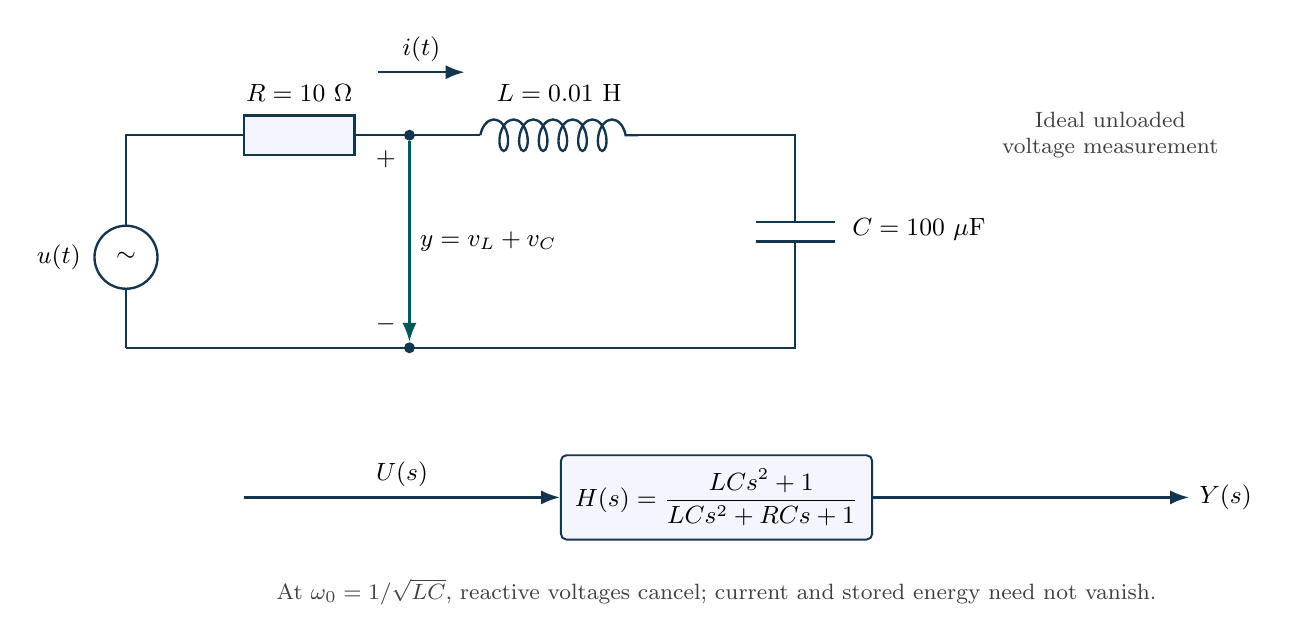
\begin{tikzpicture}[x=1cm,y=1cm,>=Latex,font=\small,
block/.style={draw=ink,fill=blue!4,rounded corners=2pt,minimum height=9mm,align=center,line width=.7pt,inner sep=5pt},
sum/.style={circle,draw=ink,fill=white,minimum size=6mm,inner sep=0pt,line width=.7pt},
sig/.style={->,draw=ink,line width=.85pt},
fb/.style={->,draw=teal!70!black,line width=.85pt},
dist/.style={->,draw=orange!75!black,line width=.85pt},
tap/.style={circle,fill=ink,inner sep=1.4pt},
note/.style={font=\footnotesize,align=center,text=black!75}]

\draw[draw=ink,line width=.85pt](.5,.3)--(.5,1.05);
\draw[draw=ink,line width=.85pt](.5,1.45)circle(.4);
\node at(.5,1.45){$\sim$};
\draw[draw=ink,line width=.85pt](.5,1.85)--(.5,3)--(2,3);
\node[left]at(.05,1.45){$u(t)$};
\draw[draw=ink,fill=blue!4,line width=.85pt](2,2.75)rectangle(3.4,3.25);
\node[above]at(2.7,3.3){$R=10\ \Omega$};
\draw[draw=ink,line width=.85pt](3.4,3)--(5,3);
\draw[decorate,decoration={coil,aspect=.55,segment length=2.5mm,amplitude=2mm},line width=.85pt,draw=ink](5,3)--(7,3);
\node[above]at(6,3.3){$L=0.01\ \mathrm{H}$};
\draw[draw=ink,line width=.85pt](7,3)--(9,3)--(9,1.9);
\draw[line width=.85pt,draw=ink](8.5,1.9)--(9.5,1.9)(8.5,1.65)--(9.5,1.65);
\draw[line width=.85pt,draw=ink](9,1.65)--(9,.3)--(.5,.3);
\node[right]at(9.6,1.8){$C=100\ \mu\mathrm{F}$};
\draw[sig](3.7,3.8)--node[above]{$i(t)$}(4.8,3.8);
\node[tap](a)at(4.1,3){};\node[tap](b)at(4.1,.3){};
\draw[fb](a)--node[right]{$y=v_L+v_C$}(b);
\node at(3.8,2.7){$+$};\node at(3.8,.6){$-$};
\node[note]at(13,3){Ideal unloaded\\voltage measurement};
\node[block](h)at(8,-1.6){$H(s)=\dfrac{LCs^2+1}{LCs^2+RCs+1}$};
\draw[sig](2,-1.6)--node[above]{$U(s)$}(h);
\draw[sig](h)--(14,-1.6)node[right]{$Y(s)$};
\node[note]at(8,-2.8){At $\omega_0=1/\sqrt{LC}$, reactive voltages cancel; current and stored energy need not vanish.};

\end{tikzpicture}
}\par{\small Series RLC network with output measured across L and C together. The output probe spans those two components, not the whole source.}\end{center}

\newpage
\section*{05. Flywheel speed regulation under a load torque}
\begin{center}\resizebox{\ifdim\width>.98\linewidth.98\linewidth\else\width\fi}{!}{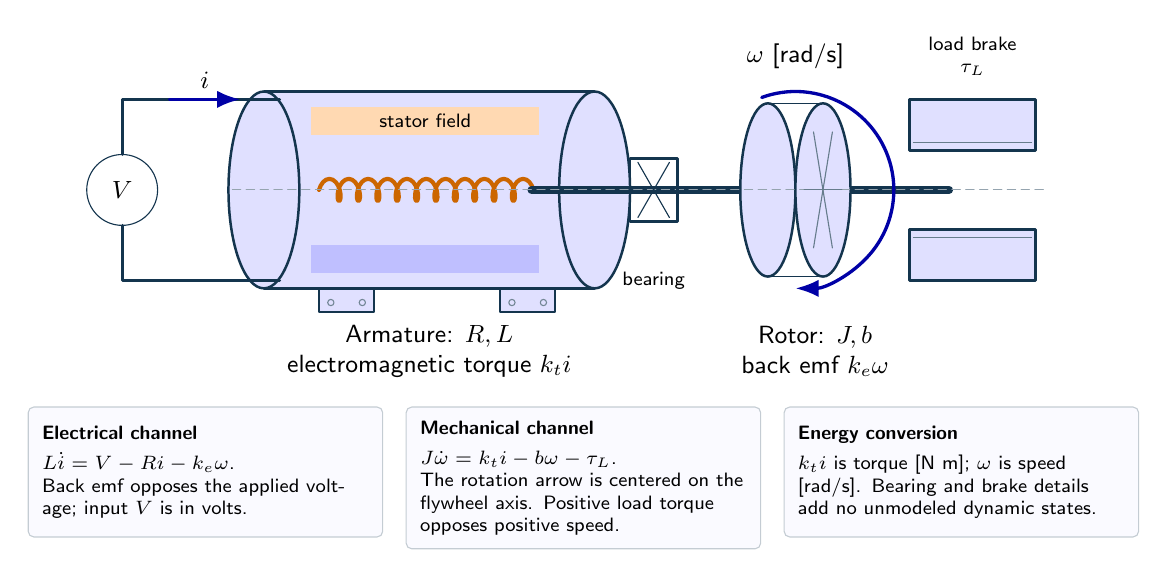
\begin{tikzpicture}[
font=\sffamily\small,>=Latex,line cap=round,line join=round,
wall/.style={draw=ink,line width=1.2pt,fill=blue!5},
water/.style={fill=cyan!25,draw=none},
metal/.style={draw=ink,fill=blue!12,line width=.9pt},
flow/.style={->,draw=blue!65!black,line width=1.2pt},
heat/.style={->,draw=orange!85!black,line width=1.1pt},
measure/.style={->,draw=teal!70!black,line width=.9pt},
dim/.style={<->,draw=ink!65,line width=.6pt},
spring/.style={draw=ink,decorate,decoration={coil,aspect=.5,segment length=4pt,amplitude=3pt}},
wire/.style={draw=ink,line width=1pt},
lab/.style={align=center,font=\sffamily\small},
smalllab/.style={align=center,font=\sffamily\scriptsize}]

\draw[metal](3,1.4)rectangle(7.2,3.9);
\draw[metal](3,2.65)ellipse(.45 and 1.25);
\draw[metal](7.2,2.65)ellipse(.45 and 1.25);
\fill[orange!30](3.6,3.35)rectangle(6.5,3.7);
\fill[blue!25](3.6,1.6)rectangle(6.5,1.95);
\node[smalllab]at(5.05,3.53){stator field};
\draw[orange!80!black,line width=1.5pt,decorate,decoration={coil,segment length=7pt,amplitude=4pt}](3.7,2.65)--(6.5,2.65);
\draw[ink,line width=3pt](6.4,2.65)--(11.7,2.65);
\draw[metal](9.4,2.65)ellipse(.35 and 1.1);
\draw[metal](10.1,2.65)ellipse(.35 and 1.1);
\draw[ink](9.4,3.75)--(10.1,3.75)(9.4,1.55)--(10.1,1.55);
\draw[metal](11.2,1.5)rectangle(12.8,2.15);
\draw[metal](11.2,3.15)rectangle(12.8,3.8);
\node[smalllab]at(12,4.35){load brake\\$\tau_L$};
\draw[flow]($(9.75,2.65)+(110:1.25)$)arc[start angle=110,end angle=-90,radius=1.25];
\node[lab]at(9.75,4.35){$\omega$ [rad/s]};
\draw[wire](3.2,3.8)--(1.2,3.8)--(1.2,3.1)(3.2,1.5)--(1.2,1.5)--(1.2,2.2);
\draw[ink](1.2,2.65)circle(.45);
\node at(1.2,2.65){$V$};
\draw[flow](1.8,3.8)--(2.7,3.8)node[midway,above]{$i$};
\node[lab]at(5.1,.6){Armature: $R,L$\\electromagnetic torque $k_t i$};
\node[lab]at(10,.6){Rotor: $J,b$\\back emf $k_e\omega$};
% REFINED EQUIPMENT DETAILS

% Motor feet, bearing blocks, shaft centerline and flywheel spokes.
\draw[metal](3.7,1.1)rectangle(4.4,1.4);\draw[metal](6,1.1)rectangle(6.7,1.4);
\foreach \x in {3.85,4.25,6.15,6.55}{\draw[ink!60](\x,1.22)circle(.04);}
\draw[ink!45,densely dashed](2.6,2.65)--(12.9,2.65);
\draw[metal,fill=none](7.65,2.25)rectangle(8.25,3.05);
\draw[ink](7.75,2.3)--(8.15,3)(7.75,3)--(8.15,2.3);
\foreach \a in {0,60,...,300}{\draw[ink!65](10.1,2.65)--++({.24*cos(\a)},{.85*sin(\a)});}
\draw[ink!65](11.25,3.25)--(12.75,3.25)(11.25,2.05)--(12.75,2.05);
\node[smalllab]at(7.95,1.5){bearing};

\node[draw=ink!25,fill=blue!2,rounded corners=2pt,anchor=north west,text width=4.15cm,minimum height=1.65cm,inner sep=5pt,align=left,font=\sffamily\scriptsize]at(0.0,-0.1){\textbf{Electrical channel}\\[3pt]$L\dot i=V-Ri-k_e\omega$.\\Back emf opposes the applied voltage; input $V$ is in volts.};
\node[draw=ink!25,fill=blue!2,rounded corners=2pt,anchor=north west,text width=4.15cm,minimum height=1.65cm,inner sep=5pt,align=left,font=\sffamily\scriptsize]at(4.8,-0.1){\textbf{Mechanical channel}\\[3pt]$J\dot\omega=k_ti-b\omega-\tau_L$.\\The rotation arrow is centered on the flywheel axis. Positive load torque opposes positive speed.};
\node[draw=ink!25,fill=blue!2,rounded corners=2pt,anchor=north west,text width=4.15cm,minimum height=1.65cm,inner sep=5pt,align=left,font=\sffamily\scriptsize]at(9.6,-0.1){\textbf{Energy conversion}\\[3pt]$k_ti$ is torque [N m]; $\omega$ is speed [rad/s]. Bearing and brake details add no unmodeled dynamic states.};
\end{tikzpicture}
}\par{\small A voltage-driven motor converts armature current into shaft torque. The rotor and external brake introduce inertia, friction and load torque. The illustrative cutaway does not add magnetic saturation or friction to the stated linear model.}\end{center}
\medskip\textbf{From equipment to equations}\par
\begin{center}\resizebox{\ifdim\width>.98\linewidth.98\linewidth\else\width\fi}{!}{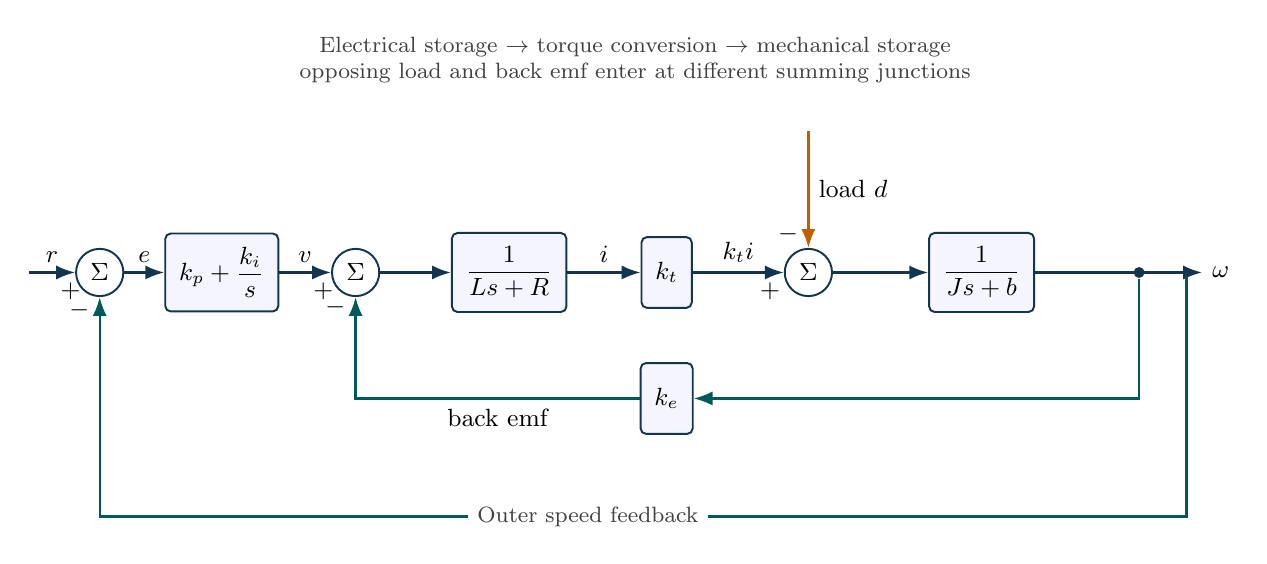
\begin{tikzpicture}[x=1cm,y=1cm,>=Latex,font=\small,
block/.style={draw=ink,fill=blue!4,rounded corners=2pt,minimum height=9mm,align=center,line width=.7pt,inner sep=5pt},
sum/.style={circle,draw=ink,fill=white,minimum size=6mm,inner sep=0pt,line width=.7pt},
sig/.style={->,draw=ink,line width=.85pt},
fb/.style={->,draw=teal!70!black,line width=.85pt},
dist/.style={->,draw=orange!75!black,line width=.85pt},
tap/.style={circle,fill=ink,inner sep=1.4pt},
note/.style={font=\footnotesize,align=center,text=black!75}]

\node[sum](e)at(.8,0){$\Sigma$};
\node[block](c)at(2.35,0){$k_p+\dfrac{k_i}{s}$};
\node[sum](v)at(4.05,0){$\Sigma$};
\node[block](el)at(6,0){$\dfrac{1}{Ls+R}$};
\node[block](kt)at(8,0){$k_t$};
\node[sum](tau)at(9.8,0){$\Sigma$};
\node[block](mech)at(12,0){$\dfrac{1}{Js+b}$};
\node[tap](w)at(14,0){};
\draw[sig](-.1,0)--node[above]{$r$}node[pos=.9,below]{$+$}(e);
\draw[sig](e)--node[above]{$e$}(c);
\draw[sig](c)--node[above]{$v$}node[pos=.85,below]{$+$}(v);
\draw[sig](v)--(el);
\draw[sig](el)--node[above]{$i$}(kt);
\draw[sig](kt)--node[above]{$k_ti$}node[pos=.85,below]{$+$}(tau);
\draw[sig](tau)--(mech);
\draw[sig](mech)--(14.8,0)node[right]{$\omega$};
\draw[dist](9.8,1.8)--node[right]{load $d$}node[pos=.88,left]{$-$}(tau);
\node[block](ke)at(8,-1.6){$k_e$};
\draw[fb](w)--(14,-1.6)--(ke);
\draw[fb](ke)--node[below]{back emf}(4.05,-1.6)--node[pos=.9,left]{$-$}(v);
\draw[fb](14.6,0)--(14.6,-3.1)--(.8,-3.1)--node[pos=.94,left]{$-$}(e);
\fill[ink](14.6,0)circle(1.4pt);
\node[note,fill=white]at(7,-3.1){Outer speed feedback};
\node[note]at(7.6,2.7){Electrical storage $\rightarrow$ torque conversion $\rightarrow$ mechanical storage\\opposing load and back emf enter at different summing junctions};

\end{tikzpicture}
}\par{\small Outer PI speed regulation around the electromechanical motor. The inner back-emf path and opposing load torque have explicit negative signs.}\end{center}

\newpage
\section*{06. Gain selection with a third-order actuator}
\begin{center}\resizebox{\ifdim\width>.98\linewidth.98\linewidth\else\width\fi}{!}{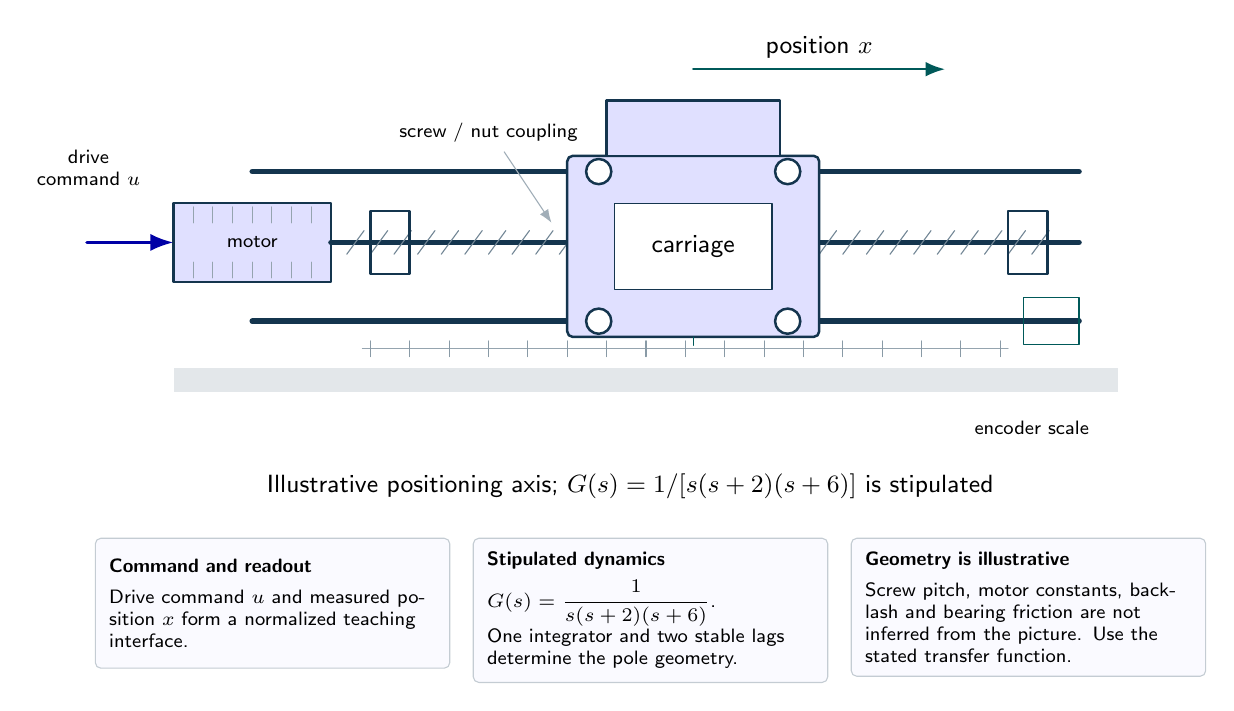
\begin{tikzpicture}[
font=\sffamily\small,>=Latex,line cap=round,line join=round,
wall/.style={draw=ink,line width=1.2pt,fill=blue!5},
water/.style={fill=cyan!25,draw=none},
metal/.style={draw=ink,fill=blue!12,line width=.9pt},
flow/.style={->,draw=blue!65!black,line width=1.2pt},
heat/.style={->,draw=orange!85!black,line width=1.1pt},
measure/.style={->,draw=teal!70!black,line width=.9pt},
dim/.style={<->,draw=ink!65,line width=.6pt},
spring/.style={draw=ink,decorate,decoration={coil,aspect=.5,segment length=4pt,amplitude=3pt}},
wire/.style={draw=ink,line width=1pt},
lab/.style={align=center,font=\sffamily\small},
smalllab/.style={align=center,font=\sffamily\scriptsize}]

\fill[ink!12](1,.5)rectangle(13,.8);
\draw[ink,line width=2pt](2,1.4)--(12.5,1.4)(2,3.3)--(12.5,3.3);
\draw[metal](1,1.9)rectangle(3,2.9);
\node[smalllab]at(2,2.4){motor};
\draw[ink,line width=2pt](3,2.4)--(12.5,2.4);
\foreach \x in {3.2,3.5,...,12.2}{\draw[ink!60](\x,2.25)--++(.22,.3);}
\draw[metal,rounded corners=2pt](6,1.2)rectangle(9.2,3.5);
\draw[fill=white,draw=ink](6.6,1.8)rectangle(8.6,2.9);
\node[lab]at(7.6,2.35){carriage};
\draw[metal](6.5,3.5)rectangle(8.7,4.2);
\draw[measure](7.6,4.6)--(10.8,4.6)node[midway,above]{position $x$};
\draw[flow](-.1,2.4)--(1,2.4);
\node[smalllab,anchor=east]at(.7,3.35){drive\\command $u$};
\draw[teal!70!black](11.8,1.1)rectangle(12.5,1.7);
\node[smalllab]at(11.9,.05){encoder scale};
\node[lab]at(6.8,-.7){Illustrative positioning axis; $G(s)=1/[s(s+2)(s+6)]$ is stipulated};
% REFINED EQUIPMENT DETAILS

% Guide bearings, screw supports and a scale tied to the carriage coordinate.
\foreach \x in {6.4,8.8}{\draw[metal,fill=white](\x,1.4)circle(.16)(\x,3.3)circle(.16);}
\draw[metal,fill=none](3.5,2)rectangle(4,2.8);\draw[metal,fill=none](11.6,2)rectangle(12.1,2.8);
\draw[ink!45](3.4,1.05)--(11.6,1.05);
\foreach \x in {3.5,4,...,11.5}{\draw[ink!50](\x,.95)--(\x,1.15);}
\draw[teal!70!black,densely dashed](7.6,1.2)--(7.6,1.05);
\foreach \x in {1.25,1.5,...,2.75}{\draw[ink!45](\x,1.95)--(\x,2.15)(\x,2.65)--(\x,2.85);}
\node[smalllab]at(5,3.8){screw / nut coupling};
\draw[ink!40,->](5.2,3.55)--(5.8,2.65);

\node[draw=ink!25,fill=blue!2,rounded corners=2pt,anchor=north west,text width=4.15cm,minimum height=1.65cm,inner sep=5pt,align=left,font=\sffamily\scriptsize]at(0.0,-1.35){\textbf{Command and readout}\\[3pt]Drive command $u$ and measured position $x$ form a normalized teaching interface.};
\node[draw=ink!25,fill=blue!2,rounded corners=2pt,anchor=north west,text width=4.15cm,minimum height=1.65cm,inner sep=5pt,align=left,font=\sffamily\scriptsize]at(4.8,-1.35){\textbf{Stipulated dynamics}\\[3pt]$G(s)=\dfrac{1}{s(s+2)(s+6)}$.\\One integrator and two stable lags determine the pole geometry.};
\node[draw=ink!25,fill=blue!2,rounded corners=2pt,anchor=north west,text width=4.15cm,minimum height=1.65cm,inner sep=5pt,align=left,font=\sffamily\scriptsize]at(9.6,-1.35){\textbf{Geometry is illustrative}\\[3pt]Screw pitch, motor constants, backlash and bearing friction are not inferred from the picture. Use the stated transfer function.};
\end{tikzpicture}
}\par{\small A motorized positioning axis illustrates the role of the integrator and two stable lags. The normalized transfer function is specified as a teaching model; the pictured dimensions do not identify its coefficients.}\end{center}
\medskip\textbf{From equipment to equations}\par
\begin{center}\resizebox{\ifdim\width>.98\linewidth.98\linewidth\else\width\fi}{!}{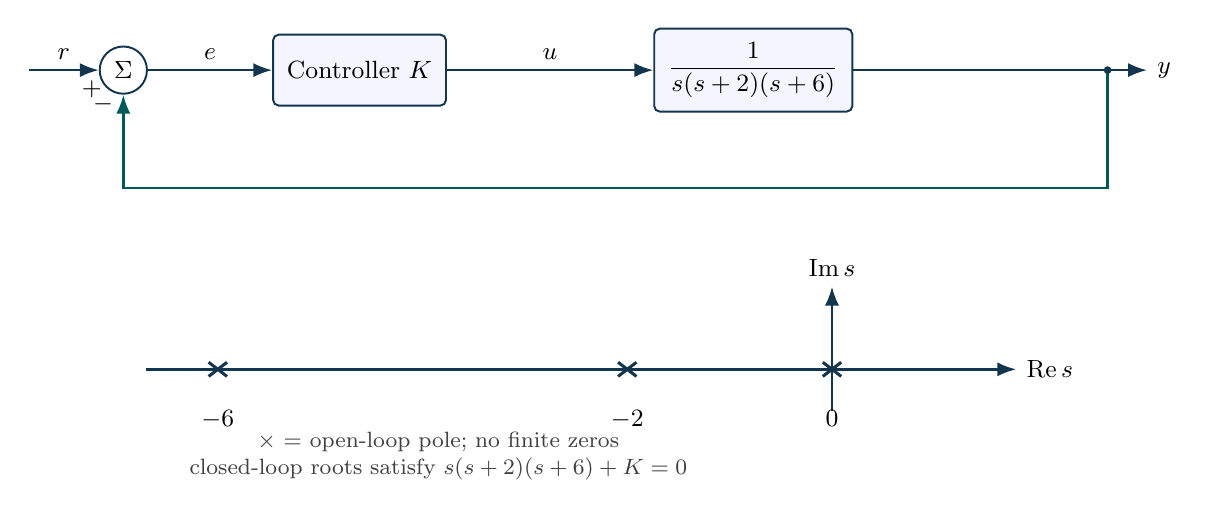
\begin{tikzpicture}[x=1cm,y=1cm,>=Latex,font=\small,
block/.style={draw=ink,fill=blue!4,rounded corners=2pt,minimum height=9mm,align=center,line width=.7pt,inner sep=5pt},
sum/.style={circle,draw=ink,fill=white,minimum size=6mm,inner sep=0pt,line width=.7pt},
sig/.style={->,draw=ink,line width=.85pt},
fb/.style={->,draw=teal!70!black,line width=.85pt},
dist/.style={->,draw=orange!75!black,line width=.85pt},
tap/.style={circle,fill=ink,inner sep=1.4pt},
note/.style={font=\footnotesize,align=center,text=black!75}]

\node[sum](e)at(1,1.8){$\Sigma$};
\node[block](k)at(4,1.8){Controller $K$};
\node[block](p)at(9,1.8){$\dfrac{1}{s(s+2)(s+6)}$};
\draw[sig](-.2,1.8)--node[above]{$r$}node[pos=.9,below]{$+$}(e);
\draw[sig](e)--node[above]{$e$}(k);
\draw[sig](k)--node[above]{$u$}(p);
\draw[sig](p)--(14,1.8)node[right]{$y$};
\draw[fb](13.5,1.8)--(13.5,.3)--(1,.3)--node[pos=.9,left]{$-$}(e);
\fill[ink](13.5,1.8)circle(1.4pt);
\begin{scope}[shift={(10,-2)},x=1.3cm,y=.75cm]
\draw[sig](-6.7,0)--(1.8,0)node[right]{$\operatorname{Re}s$};
\draw[sig](0,-.7)--(0,1.4)node[above]{$\operatorname{Im}s$};
\foreach \v in {-6,-2,0}{\draw[ink,line width=1.1pt](\v-.09,-.12)--(\v+.09,.12)(\v-.09,.12)--(\v+.09,-.12);\node[below=4mm]at(\v,0){$\v$};}
\end{scope}
\node[note]at(5,-3.1){$\times$ = open-loop pole; no finite zeros\\closed-loop roots satisfy $s(s+2)(s+6)+K=0$};

\end{tikzpicture}
}\par{\small Unity negative feedback and the open-loop pole map. Pole symbols provide the starting geometry for the root-locus exercises.}\end{center}

\newpage
\section*{07. A feedback loop with a communication delay}
\begin{center}\resizebox{\ifdim\width>.98\linewidth.98\linewidth\else\width\fi}{!}{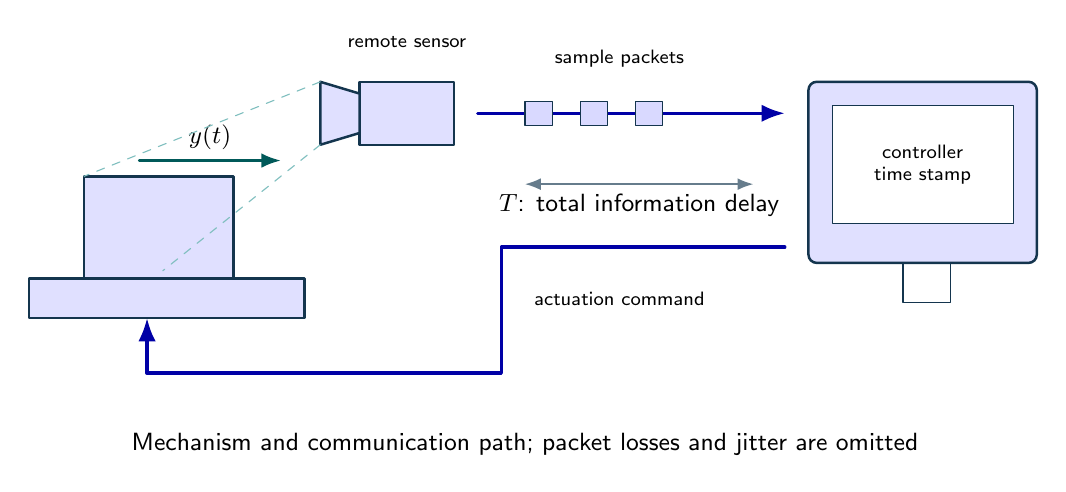
\begin{tikzpicture}[
font=\sffamily\small,>=Latex,line cap=round,line join=round,
wall/.style={draw=ink,line width=1.2pt,fill=blue!5},
water/.style={fill=cyan!25,draw=none},
metal/.style={draw=ink,fill=blue!12,line width=.9pt},
flow/.style={->,draw=blue!65!black,line width=1.2pt},
heat/.style={->,draw=orange!85!black,line width=1.1pt},
measure/.style={->,draw=teal!70!black,line width=.9pt},
dim/.style={<->,draw=ink!65,line width=.6pt},
spring/.style={draw=ink,decorate,decoration={coil,aspect=.5,segment length=4pt,amplitude=3pt}},
wire/.style={draw=ink,line width=1pt},
lab/.style={align=center,font=\sffamily\small},
smalllab/.style={align=center,font=\sffamily\scriptsize}]

\draw[metal](.5,1)rectangle(4,1.5);
\draw[metal](1.2,1.5)rectangle(3.1,2.8);
\draw[measure](1.9,3)--(3.7,3)node[midway,above]{$y(t)$};
\draw[metal](4.7,3.2)rectangle(5.9,4);
\draw[metal](4.7,3.35)--(4.2,3.2)--(4.2,4)--(4.7,3.85)--cycle;
\draw[teal!50,dashed](4.2,3.2)--(2.2,1.6)(4.2,4)--(1.2,2.8);
\node[smalllab]at(5.3,4.5){remote sensor};
\draw[metal,rounded corners=3pt](10.4,1.7)rectangle(13.3,4);
\draw[fill=white,draw=ink](10.7,2.2)rectangle(13,3.7);
\draw[ink](11.6,1.7)--(11.6,1.2)--(12.2,1.2)--(12.2,1.7);
\node[smalllab]at(11.85,2.95){controller\\time stamp};
\draw[flow](6.2,3.6)--(10.1,3.6);
\foreach \x in {6.8,7.5,8.2}{\draw[fill=blue!15,draw=ink](\x,3.45)rectangle++(.35,.3);}
\node[smalllab]at(8,4.3){sample packets};
\draw[flow](10.1,1.9)--(6.5,1.9)--(6.5,.3)--(2,.3)--(2,1);
\node[smalllab]at(8,1.25){actuation command};
\draw[dim](6.8,2.7)--node[below]{$T$: total information delay}(9.7,2.7);
\node[lab]at(6.8,-.6){Mechanism and communication path; packet losses and jitter are omitted};
\end{tikzpicture}
}\par{\small A remote mechanism sends measurements and receives commands through a communication path. The model combines those latencies into one ideal constant delay; the drawn packet train is not an experimental record.}\end{center}
\medskip\textbf{From equipment to equations}\par
\begin{center}\resizebox{\ifdim\width>.98\linewidth.98\linewidth\else\width\fi}{!}{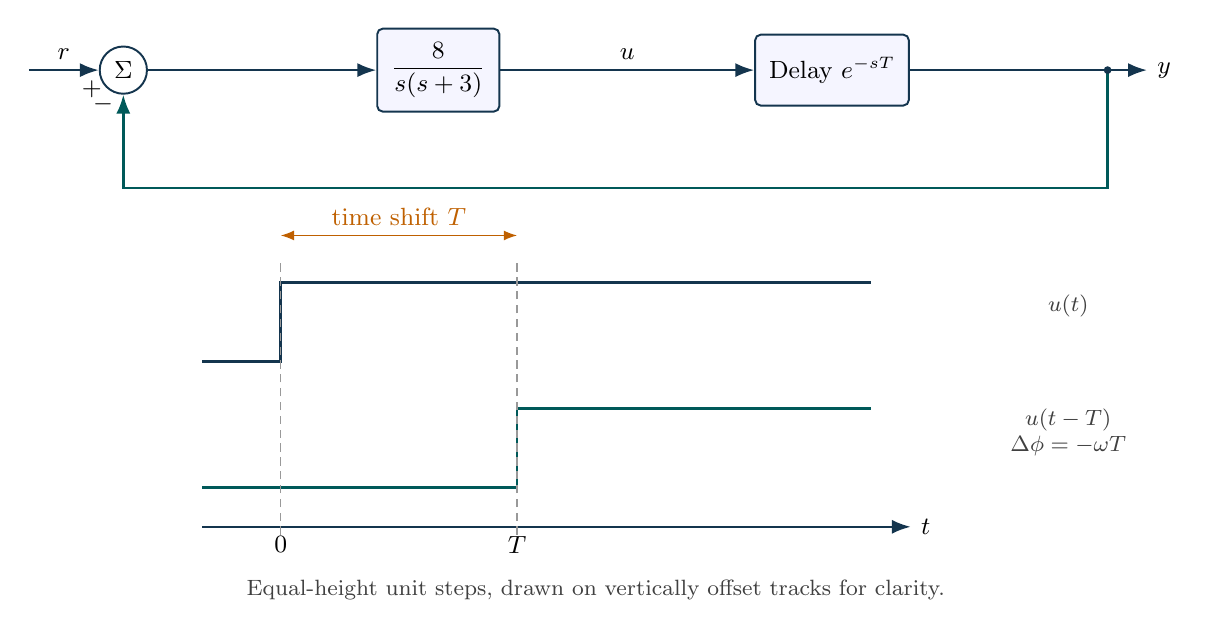
\begin{tikzpicture}[x=1cm,y=1cm,>=Latex,font=\small,
block/.style={draw=ink,fill=blue!4,rounded corners=2pt,minimum height=9mm,align=center,line width=.7pt,inner sep=5pt},
sum/.style={circle,draw=ink,fill=white,minimum size=6mm,inner sep=0pt,line width=.7pt},
sig/.style={->,draw=ink,line width=.85pt},
fb/.style={->,draw=teal!70!black,line width=.85pt},
dist/.style={->,draw=orange!75!black,line width=.85pt},
tap/.style={circle,fill=ink,inner sep=1.4pt},
note/.style={font=\footnotesize,align=center,text=black!75}]

\node[sum](e)at(1,2.1){$\Sigma$};
\node[block](g)at(5,2.1){$\dfrac{8}{s(s+3)}$};
\node[block](d)at(10,2.1){Delay $e^{-sT}$};
\draw[sig](-.2,2.1)--node[above]{$r$}node[pos=.9,below]{$+$}(e);
\draw[sig](e)--(g);\draw[sig](g)--node[above]{$u$}(d);
\draw[sig](d)--(14,2.1)node[right]{$y$};
\draw[fb](13.5,2.1)--(13.5,.6)--(1,.6)--node[pos=.9,left]{$-$}(e);
\fill[ink](13.5,2.1)circle(1.4pt);
\draw[sig](2,-3.7)--(11,-3.7)node[right]{$t$};
\draw[line width=1pt,draw=ink](2,-1.6)--(3,-1.6)--(3,-.6)--(10.5,-.6);
\draw[line width=1pt,draw=teal!70!black](2,-3.2)--(6,-3.2)--(6,-2.2)--(10.5,-2.2);
\draw[densely dashed,black!40](3,-3.8)--(3,-.35)(6,-3.8)--(6,-.35);
\node[below]at(3,-3.7){$0$};\node[below]at(6,-3.7){$T$};
\draw[<->,orange!75!black](3,0)--node[above]{time shift $T$}(6,0);
\node[note]at(13,-.9){$u(t)$};
\node[note]at(13,-2.5){$u(t-T)$\\$\Delta\phi=-\omega T$};
\node[note]at(7,-4.5){Equal-height unit steps, drawn on vertically offset tracks for clarity.};

\end{tikzpicture}
}\par{\small Constant pure delay shifts a signal in time and contributes frequency-dependent phase lag. The sketch shows ideal steps, not experimental records.}\end{center}

\newpage
\section*{08. Lead-lag design for a normalized camera axis}
\begin{center}\resizebox{\ifdim\width>.98\linewidth.98\linewidth\else\width\fi}{!}{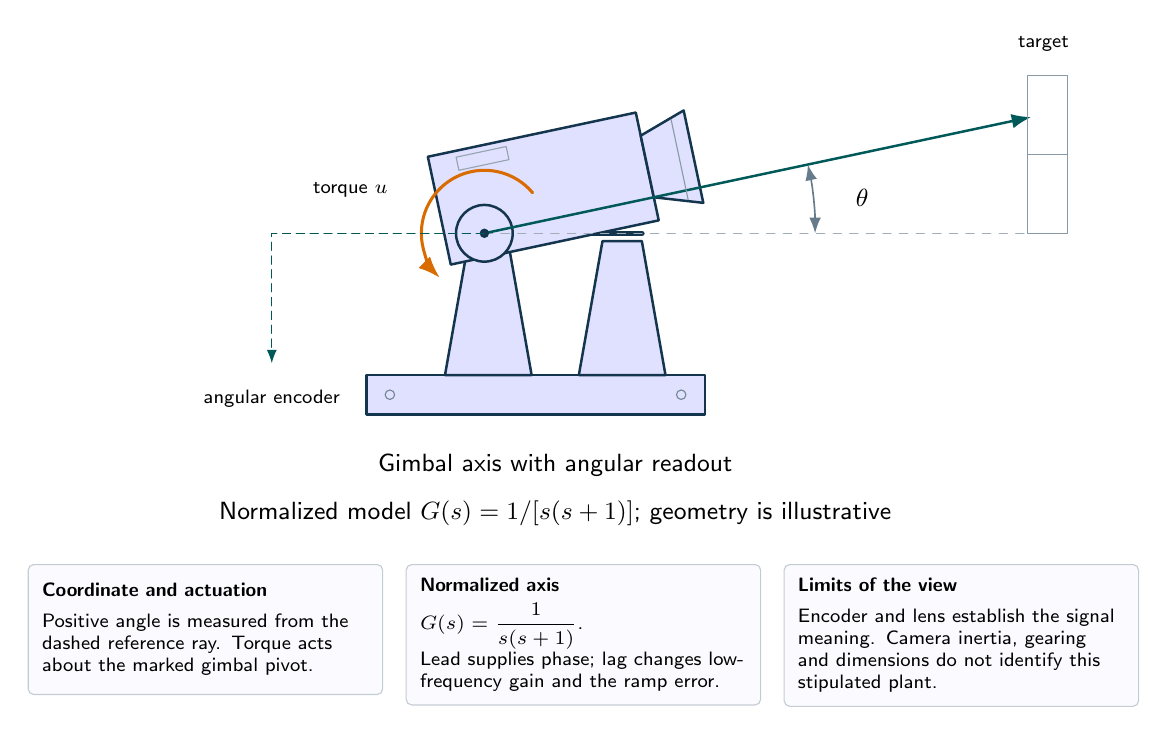
\begin{tikzpicture}[
font=\sffamily\small,>=Latex,line cap=round,line join=round,
wall/.style={draw=ink,line width=1.2pt,fill=blue!5},
water/.style={fill=cyan!25,draw=none},
metal/.style={draw=ink,fill=blue!12,line width=.9pt},
flow/.style={->,draw=blue!65!black,line width=1.2pt},
heat/.style={->,draw=orange!85!black,line width=1.1pt},
measure/.style={->,draw=teal!70!black,line width=.9pt},
dim/.style={<->,draw=ink!65,line width=.6pt},
spring/.style={draw=ink,decorate,decoration={coil,aspect=.5,segment length=4pt,amplitude=3pt}},
wire/.style={draw=ink,line width=1pt},
lab/.style={align=center,font=\sffamily\small},
smalllab/.style={align=center,font=\sffamily\scriptsize}]

\draw[metal](4.3,.4)rectangle(8.6,.9);
\draw[metal](5.3,.9)--(5.6,2.6)--(6.1,2.6)--(6.4,.9)--cycle;
\draw[metal](7,.9)--(7.3,2.6)--(7.8,2.6)--(8.1,.9)--cycle;
\draw[ink,line width=2pt](5.7,2.7)--(7.8,2.7);
\draw[metal,rotate around={12:(5.8,2.7)}](5.3,2.4)rectangle(8,3.8);
\draw[metal,rotate around={12:(5.8,2.7)}](8,2.7)--(8.6,2.5)--(8.6,3.7)--(8,3.5)--cycle;
\draw[metal](5.8,2.7)circle(.36);
\draw[heat]($(5.8,2.7)+(40:.8)$)arc[start angle=40,end angle=225,radius=.8];
\node[smalllab]at(4.1,3.25){torque $u$};
\draw[ink!40,dashed](5.8,2.7)--(12.7,2.7);
\draw[measure](5.8,2.7)--++(12:7.1);
\draw[dim]($(5.8,2.7)+(0:4.2)$)arc[start angle=0,end angle=12,radius=4.2];
\node[lab]at(10.6,3.15){$\theta$};
\draw[ink!50](12.7,2.7)rectangle(13.2,4.7);
\draw[ink!50](12.7,3.7)--(13.2,3.7);
\node[smalllab]at(12.9,5.1){target};
\node[lab]at(6.7,-.25){Gimbal axis with angular readout};
\node[lab]at(6.7,-.85){Normalized model $G(s)=1/[s(s+1)]$; geometry is illustrative};
% REFINED EQUIPMENT DETAILS

% Resolved camera lens, mounting bolts, encoder readout and pivot.
\foreach \x in {4.6,8.3}{\draw[ink!60](\x,.65)circle(.06);}
\draw[ink!50,rotate around={12:(5.8,2.7)}](8.42,2.58)--(8.42,3.62);
\draw[ink!45,rotate around={12:(5.8,2.7)}](5.65,3.55)rectangle(6.3,3.72);
\fill[ink](5.8,2.7)circle(.06);
\draw[teal!70!black,densely dashed,->](5.8,2.7)--(3.1,2.7)--(3.1,1.05);
\node[smalllab]at(3.1,.6){angular encoder};

\node[draw=ink!25,fill=blue!2,rounded corners=2pt,anchor=north west,text width=4.15cm,minimum height=1.65cm,inner sep=5pt,align=left,font=\sffamily\scriptsize]at(0.0,-1.5){\textbf{Coordinate and actuation}\\[3pt]Positive angle is measured from the dashed reference ray. Torque acts about the marked gimbal pivot.};
\node[draw=ink!25,fill=blue!2,rounded corners=2pt,anchor=north west,text width=4.15cm,minimum height=1.65cm,inner sep=5pt,align=left,font=\sffamily\scriptsize]at(4.8,-1.5){\textbf{Normalized axis}\\[3pt]$G(s)=\dfrac{1}{s(s+1)}$.\\Lead supplies phase; lag changes low-frequency gain and the ramp error.};
\node[draw=ink!25,fill=blue!2,rounded corners=2pt,anchor=north west,text width=4.15cm,minimum height=1.65cm,inner sep=5pt,align=left,font=\sffamily\scriptsize]at(9.6,-1.5){\textbf{Limits of the view}\\[3pt]Encoder and lens establish the signal meaning. Camera inertia, gearing and dimensions do not identify this stipulated plant.};
\end{tikzpicture}
}\par{\small A camera gimbal illustrates angular tracking and disturbance rejection. Its normalized plant is stipulated, with no claim that geometry alone determines its two poles.}\end{center}
\medskip\textbf{From equipment to equations}\par
\begin{center}\resizebox{\ifdim\width>.98\linewidth.98\linewidth\else\width\fi}{!}{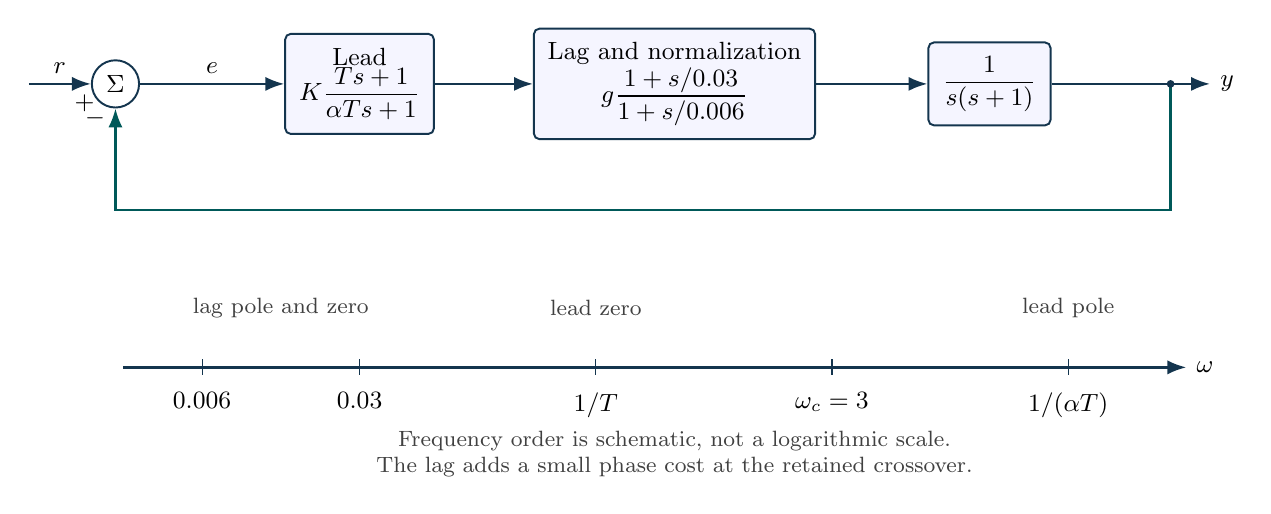
\begin{tikzpicture}[x=1cm,y=1cm,>=Latex,font=\small,
block/.style={draw=ink,fill=blue!4,rounded corners=2pt,minimum height=9mm,align=center,line width=.7pt,inner sep=5pt},
sum/.style={circle,draw=ink,fill=white,minimum size=6mm,inner sep=0pt,line width=.7pt},
sig/.style={->,draw=ink,line width=.85pt},
fb/.style={->,draw=teal!70!black,line width=.85pt},
dist/.style={->,draw=orange!75!black,line width=.85pt},
tap/.style={circle,fill=ink,inner sep=1.4pt},
note/.style={font=\footnotesize,align=center,text=black!75}]

\node[sum](e)at(.9,1.5){$\Sigma$};
\node[block](lead)at(4,1.5){Lead\\$K\dfrac{Ts+1}{\alpha Ts+1}$};
\node[block](lag)at(8,1.5){Lag and normalization\\$g\dfrac{1+s/0.03}{1+s/0.006}$};
\node[block](plant)at(12,1.5){$\dfrac{1}{s(s+1)}$};
\draw[sig](-.2,1.5)--node[above]{$r$}node[pos=.9,below]{$+$}(e);
\draw[sig](e)--node[above]{$e$}(lead);\draw[sig](lead)--(lag);\draw[sig](lag)--(plant);
\draw[sig](plant)--(14.8,1.5)node[right]{$y$};
\draw[fb](14.3,1.5)--(14.3,-.1)--(.9,-.1)--node[pos=.9,left]{$-$}(e);
\fill[ink](14.3,1.5)circle(1.4pt);
\draw[sig](1,-2.1)--(14.5,-2.1)node[right]{$\omega$};
\foreach \x/\lab in {2/0.006,4/0.03,7/{1/T},10/{\omega_c=3},13/{1/(\alpha T)}}{\draw[ink](\x,-2)--(\x,-2.2);\node[below=2mm]at(\x,-2.1){$\lab$};}
\node[note]at(3,-1.35){lag pole and zero};
\node[note]at(7,-1.35){lead zero};\node[note]at(13,-1.35){lead pole};
\node[note]at(8,-3.2){Frequency order is schematic, not a logarithmic scale.\\The lag adds a small phase cost at the retained crossover.};

\end{tikzpicture}
}\par{\small Lead and lag sections are drawn separately so their gain normalization and frequency ordering can be analyzed independently.}\end{center}

\newpage
\section*{09. PID regulation when the actuator saturates}
\begin{center}\resizebox{\ifdim\width>.98\linewidth.98\linewidth\else\width\fi}{!}{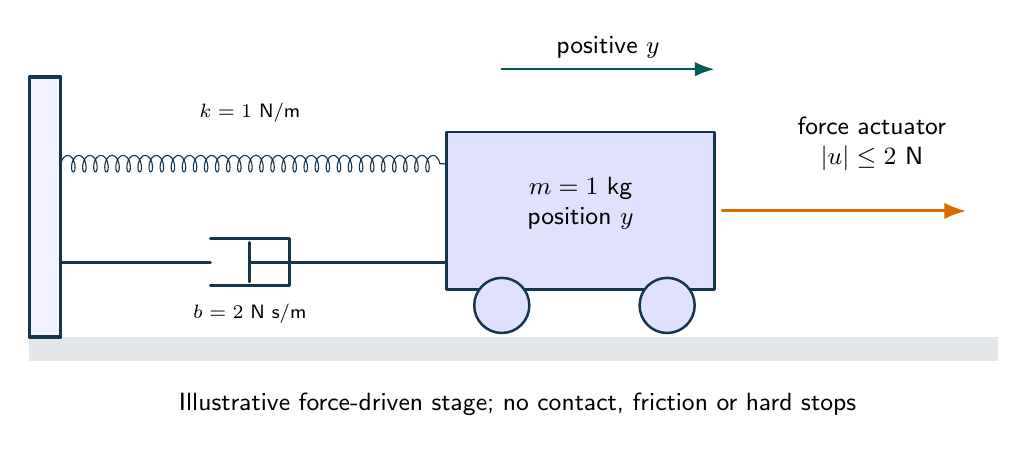
\begin{tikzpicture}[
font=\sffamily\small,>=Latex,line cap=round,line join=round,
wall/.style={draw=ink,line width=1.2pt,fill=blue!5},
water/.style={fill=cyan!25,draw=none},
metal/.style={draw=ink,fill=blue!12,line width=.9pt},
flow/.style={->,draw=blue!65!black,line width=1.2pt},
heat/.style={->,draw=orange!85!black,line width=1.1pt},
measure/.style={->,draw=teal!70!black,line width=.9pt},
dim/.style={<->,draw=ink!65,line width=.6pt},
spring/.style={draw=ink,decorate,decoration={coil,aspect=.5,segment length=4pt,amplitude=3pt}},
wire/.style={draw=ink,line width=1pt},
lab/.style={align=center,font=\sffamily\small},
smalllab/.style={align=center,font=\sffamily\scriptsize}]

\fill[ink!12](.7,.4)rectangle(13,.7);
\draw[wall](.7,.7)rectangle(1.1,4);
\draw[metal](6,1.3)rectangle(9.4,3.3);
\node[lab]at(7.7,2.4){$m=1$ kg\\position $y$};
\draw[spring](1.1,2.9)--(6,2.9);
\node[smalllab]at(3.5,3.55){$k=1$ N/m};
\draw[wire](1.1,1.65)--(3,1.65)(3,1.35)--(4,1.35)--(4,1.95)--(3,1.95);
\draw[wire](6,1.65)--(3.5,1.65)(3.5,1.4)--(3.5,1.9);
\node[smalllab]at(3.5,1){$b=2$ N s/m};
\draw[metal](6.7,1.1)circle(.35)(8.8,1.1)circle(.35);
\draw[heat](9.5,2.3)--(12.6,2.3);
\node[lab]at(11.4,3.15){force actuator\\$|u|\leq2$ N};
\draw[measure](6.7,4.1)--(9.4,4.1)node[midway,above]{positive $y$};
\node[lab]at(6.9,-.15){Illustrative force-driven stage; no contact, friction or hard stops};
\end{tikzpicture}
}\par{\small A mass, spring, damper and bounded force actuator physically realize the normalized second-order plant. Force saturation is included; contact, dry friction and travel stops are not.}\end{center}
\medskip\textbf{From equipment to equations}\par
\begin{center}\resizebox{\ifdim\width>.98\linewidth.98\linewidth\else\width\fi}{!}{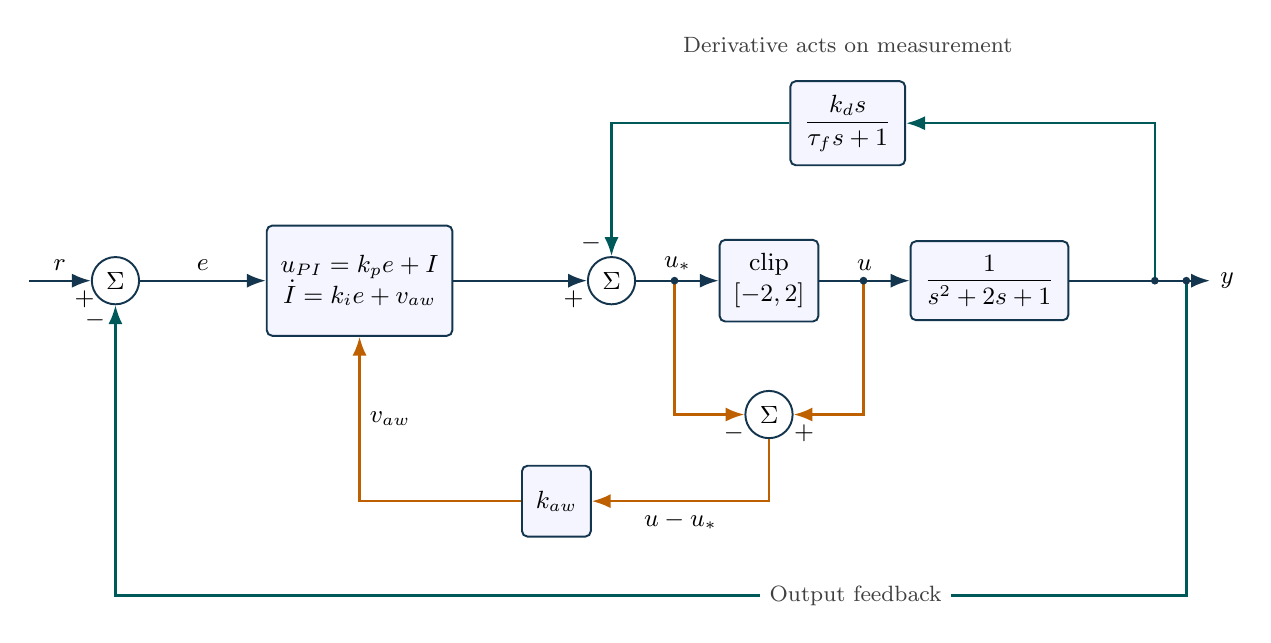
\begin{tikzpicture}[x=1cm,y=1cm,>=Latex,font=\small,
block/.style={draw=ink,fill=blue!4,rounded corners=2pt,minimum height=9mm,align=center,line width=.7pt,inner sep=5pt},
sum/.style={circle,draw=ink,fill=white,minimum size=6mm,inner sep=0pt,line width=.7pt},
sig/.style={->,draw=ink,line width=.85pt},
fb/.style={->,draw=teal!70!black,line width=.85pt},
dist/.style={->,draw=orange!75!black,line width=.85pt},
tap/.style={circle,fill=ink,inner sep=1.4pt},
note/.style={font=\footnotesize,align=center,text=black!75}]

\node[sum](e)at(.9,0){$\Sigma$};
\node[block,minimum height=14mm](pi)at(4,0){$u_{PI}=k_pe+I$\\$\dot I=k_ie+v_{aw}$};
\node[sum](tot)at(7.2,0){$\Sigma$};
\node[block](sat)at(9.2,0){$\operatorname{clip}$\\$[-2,2]$};
\node[block](plant)at(12,0){$\dfrac{1}{s^2+2s+1}$};
\draw[sig](-.2,0)--node[above]{$r$}node[pos=.9,below]{$+$}(e);
\draw[sig](e)--node[above]{$e$}(pi);
\draw[sig](pi)--node[pos=.9,below]{$+$}(tot);
\draw[sig](tot)--node[above]{$u_*$}(sat);
\draw[sig](sat)--node[above]{$u$}(plant);
\draw[sig](plant)--(14.8,0)node[right]{$y$};
\node[block](df)at(10.2,2){$\dfrac{k_ds}{\tau_fs+1}$};
\draw[fb](14.1,0)--(14.1,2)--(df);
\draw[fb](df)--(7.2,2)--node[pos=.9,left]{$-$}(tot);
\fill[ink](14.1,0)circle(1.4pt);
\node[note]at(10.2,3){Derivative acts on measurement};
\node[sum](aw)at(9.2,-1.7){$\Sigma$};
\draw[dist](10.4,0)--(10.4,-1.7)--node[pos=.85,below]{$+$}(aw);
\draw[dist](8,0)--(8,-1.7)--node[pos=.85,below]{$-$}(aw);
\fill[ink](10.4,0)circle(1.4pt);\fill[ink](8,0)circle(1.4pt);
\node[block](kaw)at(6.5,-2.8){$k_{aw}$};
\draw[dist](aw)--(9.2,-2.8)--node[below]{$u-u_*$}(kaw);
\draw[dist](kaw)--(4,-2.8)--node[right]{$v_{aw}$}(pi.south);
\draw[fb](14.5,0)--(14.5,-4)--(.9,-4)--node[pos=.95,left]{$-$}(e);
\fill[ink](14.5,0)circle(1.4pt);
\node[note,fill=white]at(10.3,-4){Output feedback};

\end{tikzpicture}
}\par{\small Filtered derivative acts on measurement. Back-calculation sends the actual-minus-requested actuator effort into the integral-state equation.}\end{center}

\newpage
\section*{10. Two thermal zones with one temperature measurement}
\begin{center}\resizebox{\ifdim\width>.98\linewidth.98\linewidth\else\width\fi}{!}{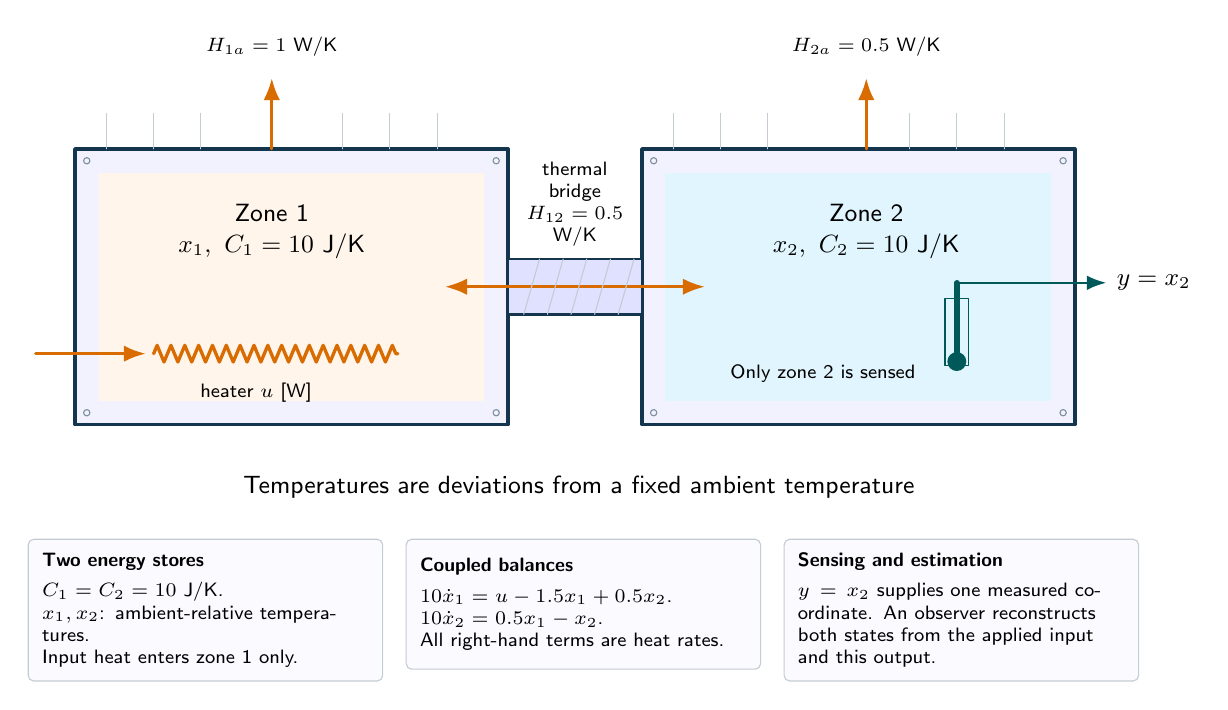
\begin{tikzpicture}[
font=\sffamily\small,>=Latex,line cap=round,line join=round,
wall/.style={draw=ink,line width=1.2pt,fill=blue!5},
water/.style={fill=cyan!25,draw=none},
metal/.style={draw=ink,fill=blue!12,line width=.9pt},
flow/.style={->,draw=blue!65!black,line width=1.2pt},
heat/.style={->,draw=orange!85!black,line width=1.1pt},
measure/.style={->,draw=teal!70!black,line width=.9pt},
dim/.style={<->,draw=ink!65,line width=.6pt},
spring/.style={draw=ink,decorate,decoration={coil,aspect=.5,segment length=4pt,amplitude=3pt}},
wire/.style={draw=ink,line width=1pt},
lab/.style={align=center,font=\sffamily\small},
smalllab/.style={align=center,font=\sffamily\scriptsize}]

\draw[wall](.6,.7)rectangle(6.1,4.2);
\draw[wall](7.8,.7)rectangle(13.3,4.2);
\fill[orange!8](.9,1)rectangle(5.8,3.9);
\fill[cyan!12](8.1,1)rectangle(13,3.9);
\draw[metal](6.1,2.1)rectangle(7.8,2.8);
\draw[heat,<->](5.3,2.45)--(8.6,2.45);
\node[smalllab]at(6.95,3.5){thermal\\bridge\\$H_{12}=0.5$\\W/K};
\draw[orange!85!black,line width=1.2pt,decorate,decoration={zigzag,segment length=5pt,amplitude=3pt}](1.6,1.6)--(4.7,1.6);
\draw[heat](.1,1.6)--(1.5,1.6);
\node[smalllab]at(2.9,1.1){heater $u$ [W]};
\node[lab]at(3.1,3.15){Zone 1\\$x_1,\ C_1=10$ J/K};
\node[lab]at(10.65,3.15){Zone 2\\$x_2,\ C_2=10$ J/K};
\draw[teal!70!black,line width=2pt](11.8,1.5)--(11.8,2.5);
\fill[teal!70!black](11.8,1.5)circle(.12);
\draw[measure](11.8,2.5)--(13.7,2.5)node[right]{$y=x_2$};
\draw[heat](3.1,4.2)--(3.1,5.1);
\draw[heat](10.65,4.2)--(10.65,5.1);
\node[smalllab]at(3.1,5.5){$H_{1a}=1$ W/K};
\node[smalllab]at(10.65,5.5){$H_{2a}=0.5$ W/K};
\node[lab]at(7,-.1){Temperatures are deviations from a fixed ambient temperature};
% REFINED EQUIPMENT DETAILS

% Distinct thermal masses and finite conductive contact.
\foreach \x in {1,1.6,2.2,4,4.6,5.2}{\draw[ink!25](\x,4.2)--(\x,4.65);}
\foreach \x in {8.2,8.8,9.4,11.2,11.8,12.4}{\draw[ink!25](\x,4.2)--(\x,4.65);}
\foreach \x in {6.3,6.6,6.9,7.2,7.5}{\draw[ink!25](\x,2.1)--(\x+.2,2.8);}
\foreach \x/\y in {.75/.85,.75/4.05,5.95/.85,5.95/4.05,7.95/.85,7.95/4.05,13.15/.85,13.15/4.05}{\draw[ink!55](\x,\y)circle(.04);}
\draw[teal!70!black](11.65,1.45)rectangle(11.95,2.3);
\node[smalllab]at(10.1,1.35){Only zone 2 is sensed};

\node[draw=ink!25,fill=blue!2,rounded corners=2pt,anchor=north west,text width=4.15cm,minimum height=1.65cm,inner sep=5pt,align=left,font=\sffamily\scriptsize]at(0.0,-0.75){\textbf{Two energy stores}\\[3pt]$C_1=C_2=10$ J/K.\\$x_1,x_2$: ambient-relative temperatures.\\Input heat enters zone 1 only.};
\node[draw=ink!25,fill=blue!2,rounded corners=2pt,anchor=north west,text width=4.15cm,minimum height=1.65cm,inner sep=5pt,align=left,font=\sffamily\scriptsize]at(4.8,-0.75){\textbf{Coupled balances}\\[3pt]$10\dot x_1=u-1.5x_1+0.5x_2$.\\$10\dot x_2=0.5x_1-x_2$.\\All right-hand terms are heat rates.};
\node[draw=ink!25,fill=blue!2,rounded corners=2pt,anchor=north west,text width=4.15cm,minimum height=1.65cm,inner sep=5pt,align=left,font=\sffamily\scriptsize]at(9.6,-0.75){\textbf{Sensing and estimation}\\[3pt]$y=x_2$ supplies one measured coordinate. An observer reconstructs both states from the applied input and this output.};
\end{tikzpicture}
}\par{\small Two thermal inventories are connected by a conductive bridge. Heating acts in the first zone and sensing in the second. These stated capacities and conductances reproduce the two-state model exactly under the lumped assumptions.}\end{center}
\medskip\textbf{From equipment to equations}\par
\begin{center}\resizebox{\ifdim\width>.98\linewidth.98\linewidth\else\width\fi}{!}{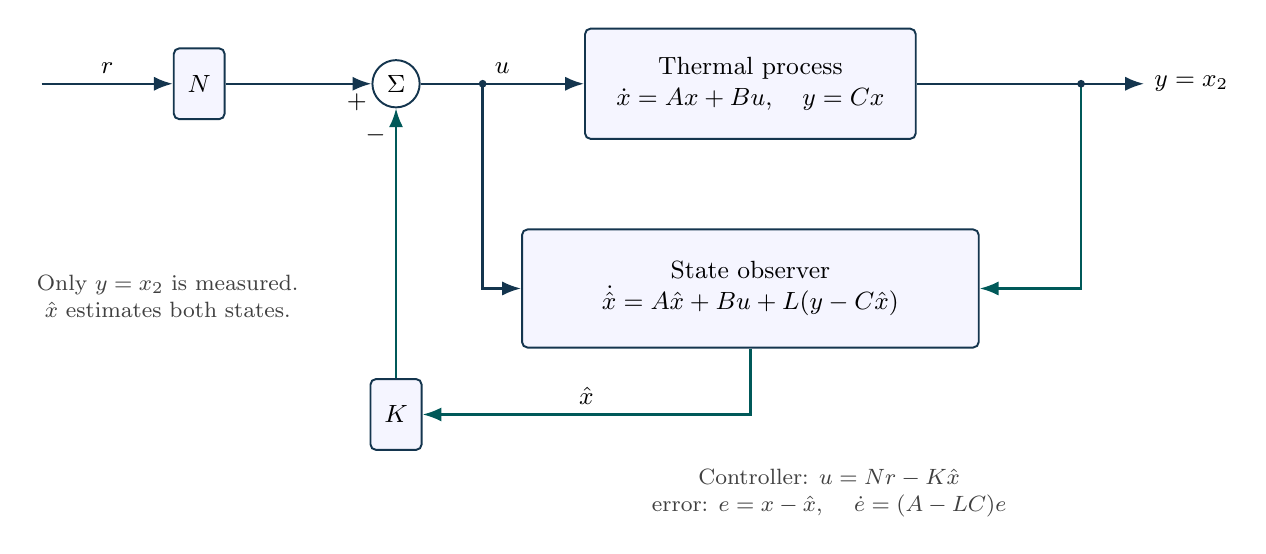
\begin{tikzpicture}[x=1cm,y=1cm,>=Latex,font=\small,
block/.style={draw=ink,fill=blue!4,rounded corners=2pt,minimum height=9mm,align=center,line width=.7pt,inner sep=5pt},
sum/.style={circle,draw=ink,fill=white,minimum size=6mm,inner sep=0pt,line width=.7pt},
sig/.style={->,draw=ink,line width=.85pt},
fb/.style={->,draw=teal!70!black,line width=.85pt},
dist/.style={->,draw=orange!75!black,line width=.85pt},
tap/.style={circle,fill=ink,inner sep=1.4pt},
note/.style={font=\footnotesize,align=center,text=black!75}]

\node[block](n)at(2,1.1){$N$};
\node[sum](u)at(4.5,1.1){$\Sigma$};
\node[block,minimum width=42mm,minimum height=14mm](p)at(9,1.1){Thermal process\\$\dot x=Ax+Bu,\quad y=Cx$};
\draw[sig](0,1.1)--node[above]{$r$}(n);
\draw[sig](n)--node[pos=.9,below]{$+$}(u);
\draw[sig](u)--node[above]{$u$}(p);
\draw[sig](p)--(14,1.1)node[right]{$y=x_2$};
\node[block,minimum width=58mm,minimum height=15mm](o)at(9,-1.5){State observer\\$\dot{\hat x}=A\hat x+Bu+L(y-C\hat x)$};
\draw[sig](5.6,1.1)--(5.6,-1.5)--(o.west);
\fill[ink](5.6,1.1)circle(1.4pt);
\draw[fb](13.2,1.1)--(13.2,-1.5)--(o.east);
\fill[ink](13.2,1.1)circle(1.4pt);
\node[block](k)at(4.5,-3.1){$K$};
\draw[fb](o.south)--(9,-3.1)--node[above]{$\hat x$}(k);
\draw[fb](k.north)--node[pos=.9,left]{$-$}(u.south);
\node[note]at(1.6,-1.6){Only $y=x_2$ is measured.\\$\hat x$ estimates both states.};
\node[note]at(10,-4.1){Controller: $u=Nr-K\hat x$\\error: $e=x-\hat x$, $\quad\dot e=(A-LC)e$};

\end{tikzpicture}
}\par{\small The observer receives both the applied control and measured output. Its estimated vector supplies state feedback; the prefilter sets nominal reference gain.}\end{center}

\newpage
\section*{11. Sampling can destabilize a continuous-time design}
\begin{center}\resizebox{\ifdim\width>.98\linewidth.98\linewidth\else\width\fi}{!}{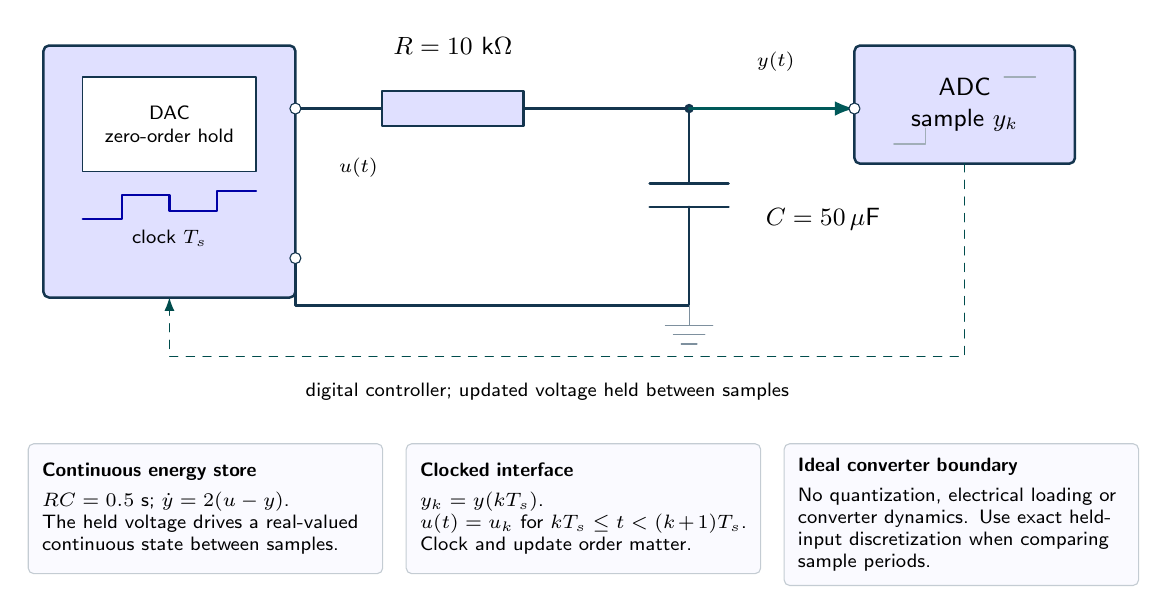
\begin{tikzpicture}[
font=\sffamily\small,>=Latex,line cap=round,line join=round,
wall/.style={draw=ink,line width=1.2pt,fill=blue!5},
water/.style={fill=cyan!25,draw=none},
metal/.style={draw=ink,fill=blue!12,line width=.9pt},
flow/.style={->,draw=blue!65!black,line width=1.2pt},
heat/.style={->,draw=orange!85!black,line width=1.1pt},
measure/.style={->,draw=teal!70!black,line width=.9pt},
dim/.style={<->,draw=ink!65,line width=.6pt},
spring/.style={draw=ink,decorate,decoration={coil,aspect=.5,segment length=4pt,amplitude=3pt}},
wire/.style={draw=ink,line width=1pt},
lab/.style={align=center,font=\sffamily\small},
smalllab/.style={align=center,font=\sffamily\scriptsize}]

\draw[metal,rounded corners=2pt](.2,1)rectangle(3.4,4.2);
\draw[fill=white,draw=ink](.7,2.6)rectangle(2.9,3.8);
\node[smalllab]at(1.8,3.2){DAC\\zero-order hold};
\node[smalllab]at(1.8,1.75){clock $T_s$};
\draw[wire](3.4,3.4)--(4.5,3.4);
\draw[metal](4.5,3.18)rectangle(6.3,3.62);
\draw[wire](6.3,3.4)--(8.4,3.4)--(8.4,2.45);
\draw[wire](7.9,2.45)--(8.9,2.45)(7.9,2.15)--(8.9,2.15);
\draw[wire](8.4,2.15)--(8.4,.9)--(3.4,.9)--(3.4,1.5);
\node[lab]at(5.4,4.2){$R=10$ k$\Omega$};
\node[lab,anchor=west]at(9.25,2.0){$C=50\,\mu$F};
\fill[ink](8.4,3.4)circle(.06);
\draw[measure](8.4,3.4)--(10.5,3.4);
\draw[metal,rounded corners=2pt](10.5,2.7)rectangle(13.3,4.2);
\node[lab]at(11.9,3.45){ADC\\sample $y_k$};
\draw[teal!60!black,dashed,->](11.9,2.7)--(11.9,.25)--(1.8,.25)--(1.8,1);
\node[smalllab]at(6.6,-.2){digital controller; updated voltage held between samples};
\node[smalllab]at(4.2,2.65){$u(t)$};
\node[smalllab]at(9.5,4){$y(t)$};
% REFINED EQUIPMENT DETAILS

% Held waveform, converter terminals and common electrical reference.
\draw[blue!65!black,line width=.8pt](.7,2)--(1.2,2)--(1.2,2.3)--(1.8,2.3)--(1.8,2.1)--(2.4,2.1)--(2.4,2.35)--(2.9,2.35);
\foreach \x/\y in {3.4/3.4,3.4/1.5,10.5/3.4}{\draw[ink,fill=white](\x,\y)circle(.07);}
\draw[ink!55](8.4,.9)--(8.4,.65)(8.1,.65)--(8.7,.65)(8.2,.53)--(8.6,.53)(8.3,.41)--(8.5,.41);
\draw[ink!40](11,2.95)--(11.4,2.95)--(11.4,3.15)(12.4,3.8)--(12.8,3.8);

\node[draw=ink!25,fill=blue!2,rounded corners=2pt,anchor=north west,text width=4.15cm,minimum height=1.65cm,inner sep=5pt,align=left,font=\sffamily\scriptsize]at(0.0,-0.85){\textbf{Continuous energy store}\\[3pt]$RC=0.5$ s; $\dot y=2(u-y)$.\\The held voltage drives a real-valued continuous state between samples.};
\node[draw=ink!25,fill=blue!2,rounded corners=2pt,anchor=north west,text width=4.15cm,minimum height=1.65cm,inner sep=5pt,align=left,font=\sffamily\scriptsize]at(4.8,-0.85){\textbf{Clocked interface}\\[3pt]$y_k=y(kT_s)$.\\$u(t)=u_k$ for $kT_s\leq t<(k+1)T_s$.\\Clock and update order matter.};
\node[draw=ink!25,fill=blue!2,rounded corners=2pt,anchor=north west,text width=4.15cm,minimum height=1.65cm,inner sep=5pt,align=left,font=\sffamily\scriptsize]at(9.6,-0.85){\textbf{Ideal converter boundary}\\[3pt]No quantization, electrical loading or converter dynamics. Use exact held-input discretization when comparing sample periods.};
\end{tikzpicture}
}\par{\small A held voltage drives an ideal RC network. The capacitor voltage is sampled by an ideal ADC; the software controller updates the DAC once per period. Quantization, converter lag and electrical loading are omitted.}\end{center}
\medskip\textbf{From equipment to equations}\par
\begin{center}\resizebox{\ifdim\width>.98\linewidth.98\linewidth\else\width\fi}{!}{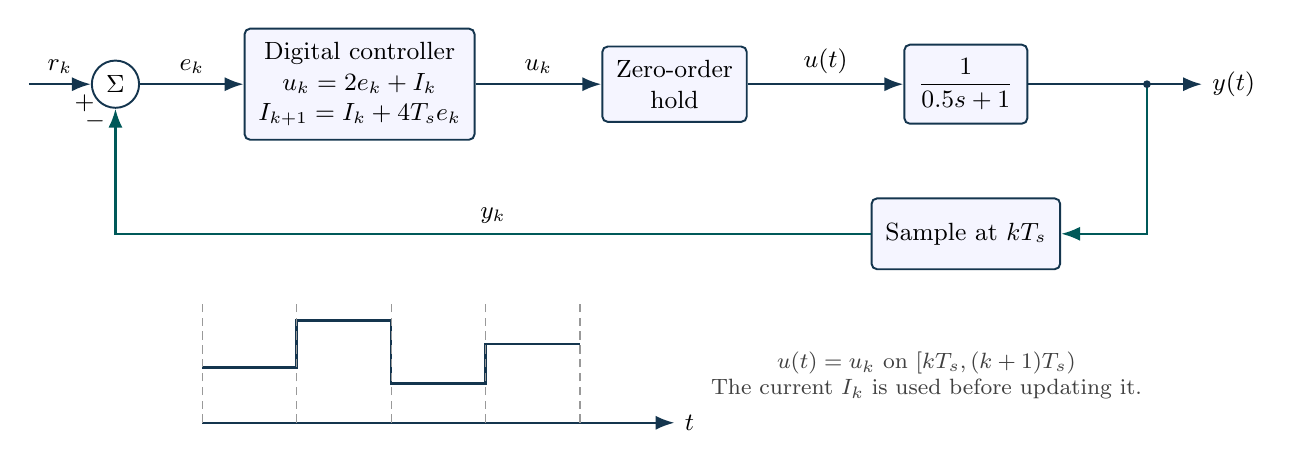
\begin{tikzpicture}[x=1cm,y=1cm,>=Latex,font=\small,
block/.style={draw=ink,fill=blue!4,rounded corners=2pt,minimum height=9mm,align=center,line width=.7pt,inner sep=5pt},
sum/.style={circle,draw=ink,fill=white,minimum size=6mm,inner sep=0pt,line width=.7pt},
sig/.style={->,draw=ink,line width=.85pt},
fb/.style={->,draw=teal!70!black,line width=.85pt},
dist/.style={->,draw=orange!75!black,line width=.85pt},
tap/.style={circle,fill=ink,inner sep=1.4pt},
note/.style={font=\footnotesize,align=center,text=black!75}]

\node[sum](e)at(.9,1.5){$\Sigma$};
\node[block,minimum height=14mm](c)at(4,1.5){Digital controller\\$u_k=2e_k+I_k$\\$I_{k+1}=I_k+4T_se_k$};
\node[block](zoh)at(8,1.5){Zero-order\\hold};
\node[block](p)at(11.7,1.5){$\dfrac{1}{0.5s+1}$};
\draw[sig](-.2,1.5)--node[above]{$r_k$}node[pos=.9,below]{$+$}(e);
\draw[sig](e)--node[above]{$e_k$}(c);
\draw[sig](c)--node[above]{$u_k$}(zoh);
\draw[sig](zoh)--node[above]{$u(t)$}(p);
\draw[sig](p)--(14.7,1.5)node[right]{$y(t)$};
\node[block](sam)at(11.7,-.4){Sample at $kT_s$};
\draw[fb](14,1.5)--(14,-.4)--(sam);
\fill[ink](14,1.5)circle(1.4pt);
\draw[fb](sam)--node[above]{$y_k$}(.9,-.4)--node[pos=.9,left]{$-$}(e);
\draw[sig](2,-2.8)--(8,-2.8)node[right]{$t$};
\draw[line width=1pt,draw=ink](2,-2.1)--(3.2,-2.1)--(3.2,-1.5)--(4.4,-1.5)--(4.4,-2.3)--(5.6,-2.3)--(5.6,-1.8)--(6.8,-1.8);
\foreach \x in{2,3.2,4.4,5.6,6.8}{\draw[black!40,densely dashed](\x,-2.8)--(\x,-1.25);}
\node[note]at(11.2,-2.2){$u(t)=u_k$ on $[kT_s,(k+1)T_s)$\\The current $I_k$ is used before updating it.};

\end{tikzpicture}
}\par{\small The sampler, digital update order and hold are explicit. Continuous plant dynamics and sampled controller states occupy different parts of the loop.}\end{center}

\newpage
\section*{12. A synthetic process from identification to validation}
\begin{center}\resizebox{\ifdim\width>.98\linewidth.98\linewidth\else\width\fi}{!}{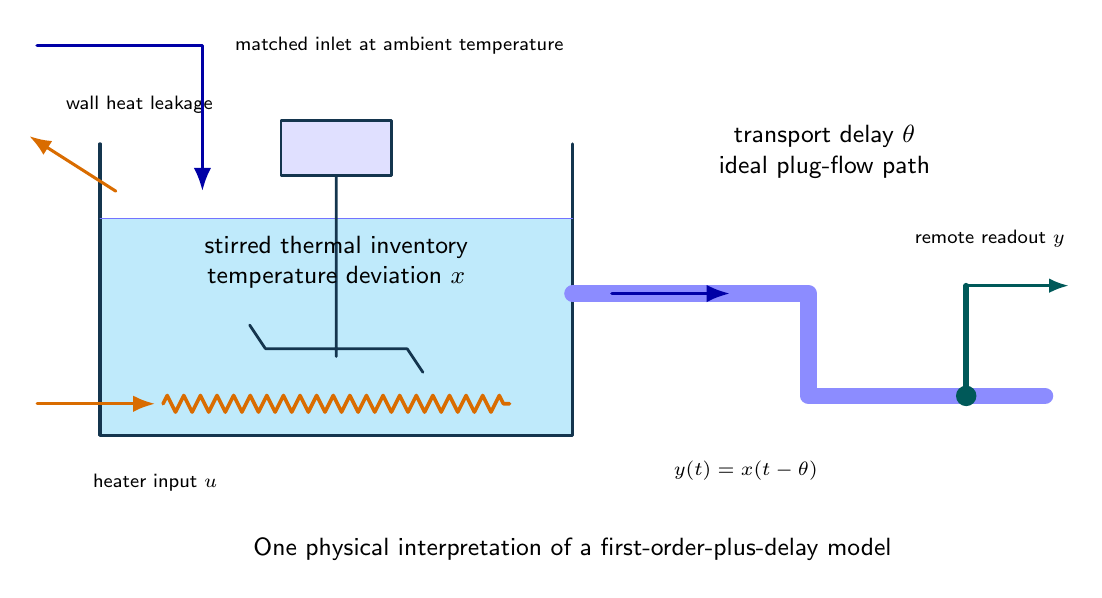
\begin{tikzpicture}[
font=\sffamily\small,>=Latex,line cap=round,line join=round,
wall/.style={draw=ink,line width=1.2pt,fill=blue!5},
water/.style={fill=cyan!25,draw=none},
metal/.style={draw=ink,fill=blue!12,line width=.9pt},
flow/.style={->,draw=blue!65!black,line width=1.2pt},
heat/.style={->,draw=orange!85!black,line width=1.1pt},
measure/.style={->,draw=teal!70!black,line width=.9pt},
dim/.style={<->,draw=ink!65,line width=.6pt},
spring/.style={draw=ink,decorate,decoration={coil,aspect=.5,segment length=4pt,amplitude=3pt}},
wire/.style={draw=ink,line width=1pt},
lab/.style={align=center,font=\sffamily\small},
smalllab/.style={align=center,font=\sffamily\scriptsize}]

\fill[water](1,.7)rectangle(7,3.45);
\draw[wall,fill=none](1,4.4)--(1,.7)--(7,.7)--(7,4.4);
\draw[blue!55](1,3.45)--(7,3.45);
\draw[metal](3.3,4)rectangle(4.7,4.7);
\draw[wire](4,4)--(4,1.7)(3.1,1.8)--(4.9,1.8)(3.1,1.8)--(2.9,2.1)(4.9,1.8)--(5.1,1.5);
\draw[orange!85!black,line width=1.3pt,decorate,decoration={zigzag,segment length=6pt,amplitude=3pt}](1.8,1.1)--(6.2,1.1);
\draw[heat](.2,1.1)--(1.7,1.1);
\node[smalllab]at(1.7,.1){heater input $u$};
\node[lab]at(4,2.9){stirred thermal inventory\\temperature deviation $x$};
\draw[heat](1.2,3.8)--(.1,4.5);
\node[smalllab]at(1.5,4.9){wall heat leakage};
\draw[flow](.2,5.65)--(2.3,5.65)--(2.3,3.8);
\node[smalllab]at(4.8,5.65){matched inlet at ambient temperature};
\draw[blue!45,line width=6pt](7,2.5)--(10,2.5)--(10,1.2)--(13,1.2);
\draw[flow](7.5,2.5)--(9,2.5);
\draw[teal!70!black,line width=2pt](12,1.2)--(12,2.6);
\fill[teal!70!black](12,1.2)circle(.13);
\draw[measure](12,2.6)--(13.3,2.6);
\node[smalllab]at(12.3,3.2){remote readout $y$};
\node[lab]at(10.2,4.3){transport delay $\theta$\\ideal plug-flow path};
\node[smalllab]at(9.2,.25){$y(t)=x(t-\theta)$};
\node[lab]at(7,-.75){One physical interpretation of a first-order-plus-delay model};
\end{tikzpicture}
}\par{\small A stirred thermal inventory followed by ideal transport is one possible physical interpretation of the identified transfer function. The effective conductance includes wall leakage and through-flow heat removal. Its fitted gain and time constant do not separately determine capacity, conductance and heater efficiency.}\end{center}
\medskip\textbf{From equipment to equations}\par
\begin{center}\resizebox{\ifdim\width>.98\linewidth.98\linewidth\else\width\fi}{!}{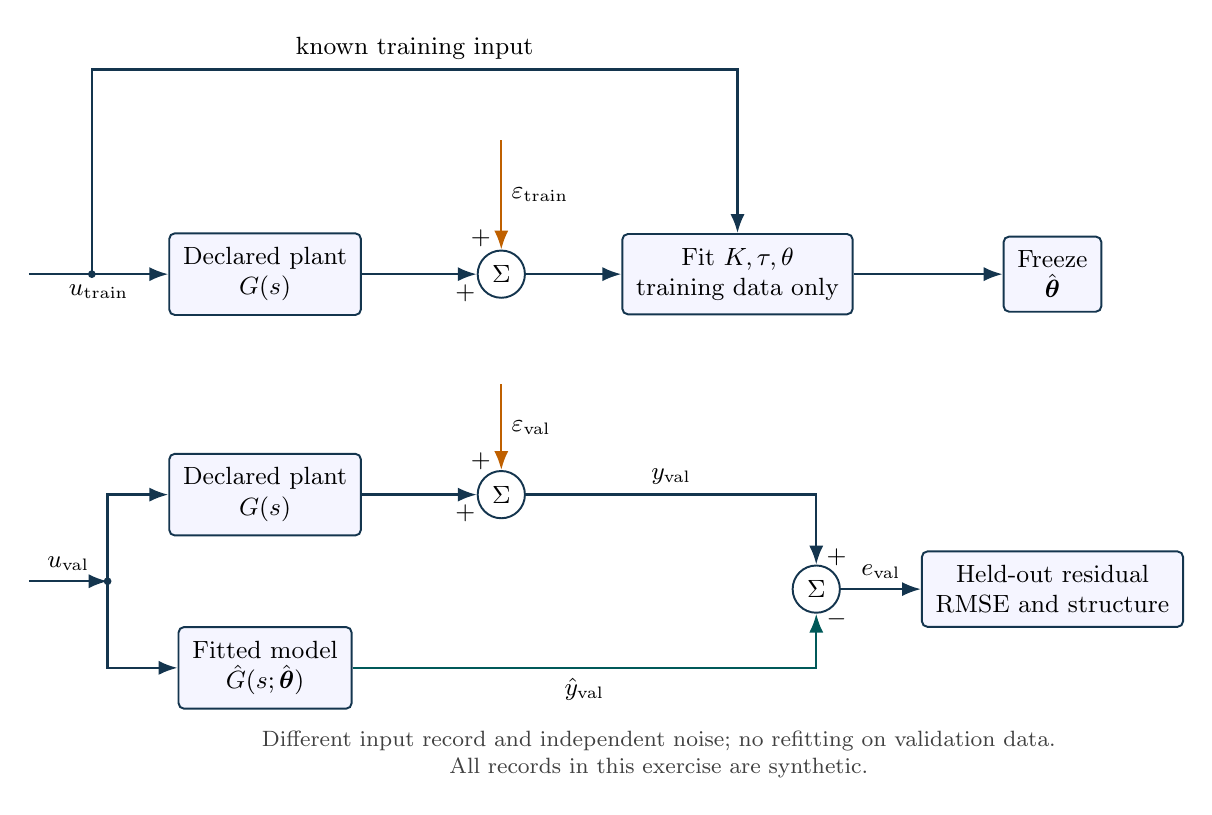
\begin{tikzpicture}[x=1cm,y=1cm,>=Latex,font=\small,
block/.style={draw=ink,fill=blue!4,rounded corners=2pt,minimum height=9mm,align=center,line width=.7pt,inner sep=5pt},
sum/.style={circle,draw=ink,fill=white,minimum size=6mm,inner sep=0pt,line width=.7pt},
sig/.style={->,draw=ink,line width=.85pt},
fb/.style={->,draw=teal!70!black,line width=.85pt},
dist/.style={->,draw=orange!75!black,line width=.85pt},
tap/.style={circle,fill=ink,inner sep=1.4pt},
note/.style={font=\footnotesize,align=center,text=black!75}]

\node[block](plant)at(3,1.5){Declared plant\\$G(s)$};
\node[sum](noise)at(6,1.5){$\Sigma$};
\node[block](fit)at(9,1.5){Fit $K,\tau,\theta$\\training data only};
\node[block](freeze)at(13,1.5){Freeze\\$\hat{\boldsymbol\theta}$};
\draw[sig](0,1.5)--node[below]{$u_{\mathrm{train}}$}(plant);
\draw[sig](plant)--node[pos=.9,below]{$+$}(noise);
\draw[dist](6,3.2)--node[right]{$\varepsilon_{\mathrm{train}}$}node[pos=.9,left]{$+$}(noise);
\draw[sig](noise)--(fit);\draw[sig](fit)--(freeze);
\draw[sig](.8,1.5)--(.8,4.1)--node[above]{known training input}(9,4.1)--(fit.north);
\fill[ink](.8,1.5)circle(1.4pt);
\node[block](truth)at(3,-1.3){Declared plant\\$G(s)$};
\node[block](pred)at(3,-3.5){Fitted model\\$\hat G(s;\hat{\boldsymbol\theta})$};
\node[sum](nv)at(6,-1.3){$\Sigma$};
\node[sum](err)at(10,-2.5){$\Sigma$};
\node[block](metric)at(13,-2.5){Held-out residual\\RMSE and structure};
\draw[sig](0,-2.4)--node[above]{$u_{\mathrm{val}}$}(1,-2.4);
\draw[sig](1,-2.4)--(1,-1.3)--(truth);
\draw[sig](1,-2.4)--(1,-3.5)--(pred);
\fill[ink](1,-2.4)circle(1.4pt);
\draw[sig](truth)--node[pos=.9,below]{$+$}(nv);
\draw[dist](6,.1)--node[right]{$\varepsilon_{\mathrm{val}}$}node[pos=.9,left]{$+$}(nv);
\draw[sig](nv)--node[above]{$y_{\mathrm{val}}$}(10,-1.3)--node[pos=.9,right]{$+$}(err);
\draw[fb](pred)--node[below]{$\hat y_{\mathrm{val}}$}(10,-3.5)--node[pos=.9,right]{$-$}(err);
\draw[sig](err)--node[above]{$e_{\mathrm{val}}$}(metric);
\node[note]at(8,-4.6){Different input record and independent noise; no refitting on validation data.\\All records in this exercise are synthetic.};

\end{tikzpicture}
}\par{\small Training selects parameters; held-out validation freezes them. Separate noise records avoid reusing training residuals as validation evidence.}\end{center}

\newpage
\section*{Integrated study: interacting water tanks}
Two open tanks have constant areas $A_1=0.02$ m$^2$ and $A_2=0.03$ m$^2$. Their submerged connection obeys
\[
q_{12}=k_{12}\operatorname{sgn}(h_1-h_2)\sqrt{|h_1-h_2|},\qquad
q_2=k_2\sqrt{h_2},
\]
where $k_{12}=0.004$ and $k_2=0.003$ m$^{5/2}$/s. The pump feeds only tank 1. Nominal inflow is $\bar q=0.0012$ m$^3$/s; the measured output is $h_2$. Areas and discharge coefficients are hypothetical. Assume nonnegative levels, no overflow and ideal sensing.
\begin{center}\resizebox{\ifdim\width>.98\linewidth.98\linewidth\else\width\fi}{!}{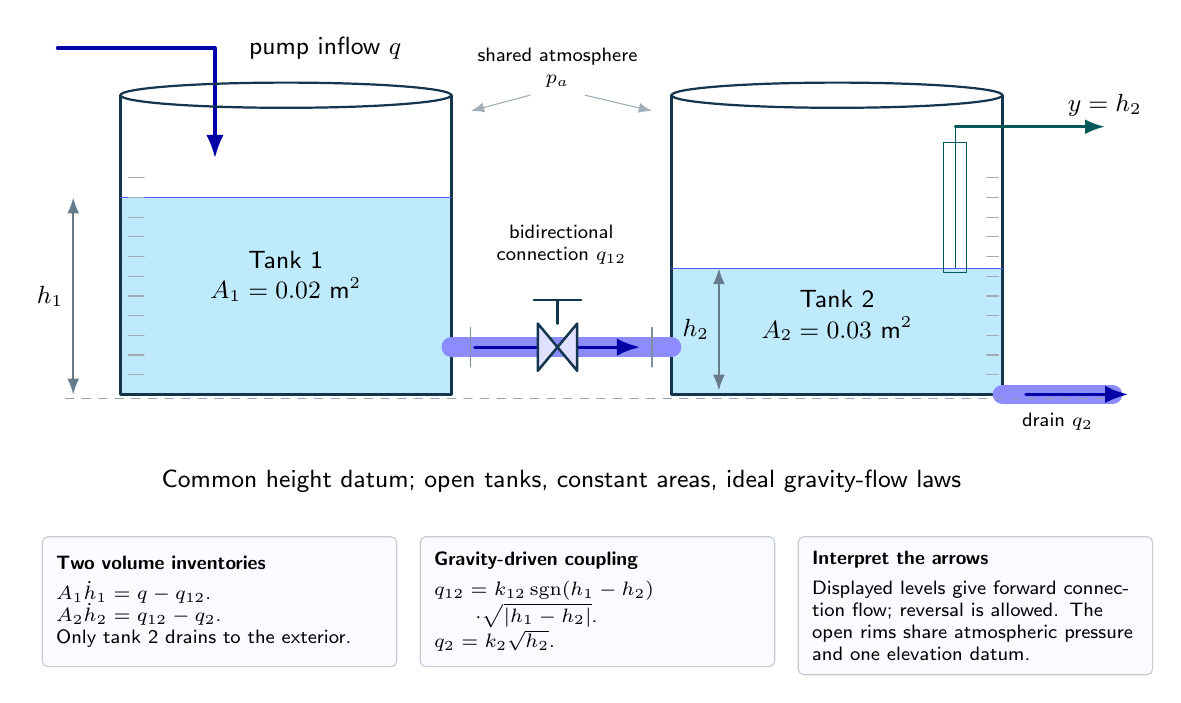
\begin{tikzpicture}[
font=\sffamily\small,>=Latex,line cap=round,line join=round,
wall/.style={draw=ink,line width=1.2pt,fill=blue!5},
water/.style={fill=cyan!25,draw=none},
metal/.style={draw=ink,fill=blue!12,line width=.9pt},
flow/.style={->,draw=blue!65!black,line width=1.2pt},
heat/.style={->,draw=orange!85!black,line width=1.1pt},
measure/.style={->,draw=teal!70!black,line width=.9pt},
dim/.style={<->,draw=ink!65,line width=.6pt},
spring/.style={draw=ink,decorate,decoration={coil,aspect=.5,segment length=4pt,amplitude=3pt}},
wire/.style={draw=ink,line width=1pt},
lab/.style={align=center,font=\sffamily\small},
smalllab/.style={align=center,font=\sffamily\scriptsize}]

\fill[water](1,1)rectangle(5.2,3.5);
\fill[water](8,1)rectangle(12.2,2.6);
\draw[wall,fill=none](1,4.8)--(1,1)--(5.2,1)--(5.2,4.8);
\draw[wall,fill=none](8,4.8)--(8,1)--(12.2,1)--(12.2,4.8);
\draw[blue!65](1,3.5)--(5.2,3.5)(8,2.6)--(12.2,2.6);
\draw[blue!45,line width=7pt](5.2,1.6)--(8,1.6);
\draw[blue!45,line width=7pt](12.2,1)--(13.6,1);
\draw[flow](5.5,1.6)--(7.6,1.6);
\draw[flow](12.5,1)--(13.8,1);
\draw[metal](6.3,1.3)--(6.8,1.9)--(6.8,1.3)--(6.3,1.9)--cycle;
\draw[wire](6.55,1.9)--(6.55,2.2)(6.25,2.2)--(6.85,2.2);
\node[smalllab]at(6.6,2.9){bidirectional\\connection $q_{12}$};
\node[smalllab]at(12.9,.65){drain $q_2$};
\draw[flow](.2,5.4)--(2.2,5.4)--(2.2,4);
\node[lab]at(3.6,5.4){pump inflow $q$};
\node[lab]at(3.1,2.5){Tank 1\\$A_1=0.02$ m$^2$};
\node[lab]at(10.1,2){Tank 2\\$A_2=0.03$ m$^2$};
\draw[dim](.4,1)--node[left]{$h_1$}(.4,3.5);
\draw[dim](8.6,1.05)--node[left]{$h_2$}(8.6,2.6);
\draw[teal!70!black](11.6,2.6)--(11.6,4.4);
\draw[measure](11.6,4.4)--(13.5,4.4)node[above]{$y=h_2$};
\draw[ink!45,dashed](.3,.95)--(13.5,.95);
\node[lab]at(6.6,-.1){Common height datum; open tanks, constant areas, ideal gravity-flow laws};
% REFINED EQUIPMENT DETAILS

% Open tank rims, submerged ports and an instrument associated with h2.
\draw[ink,line width=.8pt](3.1,4.8)ellipse(2.1 and .16);
\draw[ink,line width=.8pt](10.1,4.8)ellipse(2.1 and .16);
\foreach \x in {5.45,7.75}{\draw[ink!55](\x,1.35)--(\x,1.85);}
\draw[teal!70!black](11.45,2.55)rectangle(11.75,4.2);
\foreach \y in {1.25,1.5,...,3.75}{\draw[ink!40](1.1,\y)--(1.3,\y)(12,\y)--(12.15,\y);}
\node[smalllab]at(6.55,5.15){shared atmosphere\\$p_a$};
\draw[ink!40,->](6.2,4.8)--(5.45,4.6);\draw[ink!40,->](6.9,4.8)--(7.75,4.6);

\node[draw=ink!25,fill=blue!2,rounded corners=2pt,anchor=north west,text width=4.15cm,minimum height=1.65cm,inner sep=5pt,align=left,font=\sffamily\scriptsize]at(0.0,-0.8){\textbf{Two volume inventories}\\[3pt]$A_1\dot h_1=q-q_{12}$.\\$A_2\dot h_2=q_{12}-q_2$.\\Only tank 2 drains to the exterior.};
\node[draw=ink!25,fill=blue!2,rounded corners=2pt,anchor=north west,text width=4.15cm,minimum height=1.65cm,inner sep=5pt,align=left,font=\sffamily\scriptsize]at(4.8,-0.8){\textbf{Gravity-driven coupling}\\[3pt]$q_{12}=k_{12}\operatorname{sgn}(h_1-h_2)$\\$\qquad\cdot\sqrt{|h_1-h_2|}$.\\$q_2=k_2\sqrt{h_2}$.};
\node[draw=ink!25,fill=blue!2,rounded corners=2pt,anchor=north west,text width=4.15cm,minimum height=1.65cm,inner sep=5pt,align=left,font=\sffamily\scriptsize]at(9.6,-0.8){\textbf{Interpret the arrows}\\[3pt]Displayed levels give forward connection flow; reversal is allowed. The open rims share atmospheric pressure and one elevation datum.};
\end{tikzpicture}
}\par{\small Interacting tanks share a submerged connection at a common datum. Flow reverses if the level ordering reverses. Only tank 2 drains to the exterior; this is not a cascade with a freely falling inter-tank stream.}\end{center}
The six-part case derives conservation laws, local dynamics, finite-step error, PI stability, pump feasibility and a validation protocol.
\end{document}
